\documentclass[
  lang=cn,
  degree=bachelor,type=paper,
  openany,oneside
  % openright,blankleft,twoside
]{nuaathesis}

\graphicspath{{./fig/},{./logo/},{../logo/}}

\iffalse
  % 本块代码被上方的 iffalse 注释掉,如需使用,请改为 iftrue
  % 使用 Noto 字体替换中文宋体、黑体
  \setCJKfamilyfont{\CJKrmdefault}[BoldFont=Noto Serif CJK SC Bold]{Noto Serif CJK SC}
  \renewcommand\songti{\CJKfamily{\CJKrmdefault}}
  \setCJKfamilyfont{\CJKsfdefault}[BoldFont=Noto Sans CJK SC Bold]{Noto Sans CJK SC Medium}
  \renewcommand\heiti{\CJKfamily{\CJKsfdefault}}
\fi

\iffalse
  % 本块代码被上方的 iffalse 注释掉,如需使用,请改为 iftrue
  % 在 XeLaTeX + ctexbook 环境下使用 Noto 日文字体
  \setCJKfamilyfont{mc}[BoldFont=Noto Serif CJK JP Bold]{Noto Serif CJK JP}
  \newcommand\mcfamily{\CJKfamily{mc}}
  \setCJKfamilyfont{gt}[BoldFont=Noto Sans CJK JP Bold]{Noto Sans CJK JP}
  \newcommand\gtfamily{\CJKfamily{gt}}
\fi

\iftrue
  % 使用微软字体替换中文宋体、黑体、楷体
  \setCJKfamilyfont{\CJKrmdefault}[AutoFakeBold]{SimSun}
  \renewcommand\songti{\CJKfamily{\CJKrmdefault}}
  \setCJKfamilyfont{\CJKsfdefault}[AutoFakeBold]{SimHei}
  \renewcommand\heiti{\CJKfamily{\CJKsfdefault}}
  \setCJKfamilyfont{kai}[AutoFakeBold]{KaiTi}
  \renewcommand\kaishu{\CJKfamily{kai}}

\fi

% 设置基本文档信息,\linebreak 前面不要有空格,否则在无需换行的场合,中文之间的空格无法消除
\nuaaset{
  title = {结合度量学习的鲁棒神经网络研究和实现},
  author = {陶略},
  college = {计算机科学与技术学院},
  advisers = {陈松灿},
  % applydate = {二〇一八年六月}  % 默认当前日期
  %
  % 本科
  major = {计算机科学与技术},
  studentid = {031510319},
  classid = {1615102},
  % 硕/博士
  majorsubject = {\LaTeX},
  researchfield = {\LaTeX 排版},
  libraryclassid = {TP371},       % 中图分类号
  subjectclassid = {080605},      % 学科分类号
  thesisid = {1028704 18-S000},   % 论文编号
}
\nuaasetEn{
  title = {Research and Implementation of Robust Neural Network Based on Metric Learning},
  author = {Lue Tao},
  college = {College of Computer Science and Technology},
  majorsubject = {\LaTeX{} Typesetting},
  advisers = {Songcan Chen, tex.se users},
  % degreefull = {Master of Art and Engineering},
  % applydate = {June, 8012}
}

% 摘要
\begin{abstract}

由于在自然图像、自然语言等数据中普遍存在的层次性和非线性性,深度神经网络在诸多现实任务上都取得了巨大的进展。从已大规模部署的人脸识别系统,到正在发展阶段的自动驾驶汽车,深度学习技术正逐渐走进并将改变人类生活的各方面。虽然深度学习在通常情况下都具有较好的泛化性能,但近年来,神经网络被发现在对抗样本的攻击下,表现出了非常糟糕的性能,而这些对抗样本对人类来说与正常样本无异。这引发了人们对基于深度网络等智能系统的安全性担忧,同时也揭示了目前深度网络对周围世界的理解能力远远不及人类智能的事实。对抗训练作为一个有效的提高神经网络鲁棒性和安全性的方法已开始倍受广泛关注,但其泛化性能却难尽人意。本文工作旨在尝试结合度量学习思想,利用相关的正则化技术,以提高对抗训练的泛化性能,并通过大量的实验获得了有效性验证。

\end{abstract}
\keywords{深度学习, 神经网络,对抗样本, 鲁棒学习,度量学习, 正则化}

\begin{abstractEn}

Because of the hierarchy and non-linearity in the natural image and natural language data, deep learning has made great progress in many practical tasks. From the face recognition system that has been deployed on a large scale, to the self-driving car in the developing stage, deep learning is stepping into and changing all aspects of human life. Although deep learning usually has good generalization performance in most cases, in recent years, neural networks have been found to exhibit very poor performance against adversarial examples, which are nearly indistinguishable from the clean examples. These raise concerns about the security of intelligent systems such as deep network, and also reveal the fact that deep networks are far less capable of understanding the surrounding world than human intelligence. As an effective method to improve the robustness and security of neural networks, adversarial training has attracted much attention, but its generalization performance is unsatisfactory. The purpose of this paper is to try to improve the generalization performance of adversarial training by combining the idea of metric learning and using relevant regularization techniques. We acquire the effectiveness of regularizations by extensive experiments.

\end{abstractEn}
\keywordsEn{Deep learning, Neural network, Adversarial example, Robust learning, Metric learning, Regularization}


% 请按自己的论文排版需求,随意修改以下全局设置

\usepackage{subfig}
\usepackage{rotating}
\usepackage[usenames,dvipsnames]{xcolor}
\usepackage{tikz}
\usepackage{pgfplots}
\pgfplotsset{compat=1.16}
\pgfplotsset{
  table/search path={./fig/},
}
\usepackage{ifthen}
\usepackage{longtable}
\usepackage{siunitx}
\usepackage{listings}
\usepackage{multirow}
\usepackage[bottom]{footmisc}
\usepackage{pifont}
\usepackage{booktabs}   % For thickness of table line
\usepackage{hyperref}   % For cross-reference with custon text

\lstdefinestyle{lstStyleBase}{%
  basicstyle=\small\ttfamily,
  aboveskip=\medskipamount,
  belowskip=\medskipamount,
  lineskip=0pt,
  boxpos=c,
  showlines=false,
  extendedchars=true,
  upquote=true,
  tabsize=2,
  showtabs=false,
  showspaces=false,
  showstringspaces=false,
  numbers=left,
  numberstyle=\footnotesize,
  linewidth=\linewidth,
  xleftmargin=\parindent,
  xrightmargin=0pt,
  resetmargins=false,
  breaklines=true,
  breakatwhitespace=false,
  breakindent=0pt,
  breakautoindent=true,
  columns=flexible,
  keepspaces=true,
  framesep=3pt,
  rulesep=2pt,
  framerule=1pt,
  backgroundcolor=\color{gray!5},
  stringstyle=\color{green!40!black!100},
  keywordstyle=\bfseries\color{blue!50!black},
  commentstyle=\slshape\color{black!60}}

%\usetikzlibrary{external}
%\tikzexternalize % activate!

\newcommand\cs[1]{\texttt{\textbackslash#1}}
\newcommand\pkg[1]{\texttt{#1}\textsuperscript{PKG}}
\newcommand\env[1]{\texttt{#1}}

\theoremstyle{nuaaplain}
\nuaatheoremchapu{definition}{定义}
\nuaatheoremchapu{assumption}{假设}
\nuaatheoremchap{exercise}{练习}
\nuaatheoremchap{nonsense}{胡诌}
\nuaatheoremg[句]{lines}{句子}

% \includeonly{content/start,}

\begin{document}

\makecover
\makedeclare
\frontmatter
\makeabstract
% 如果需要调整目录层级数量的话,取消下一行注释,数字含义: 0=chapter, 1=section, 2=subsection
% \setcounter{tocdepth}{1}
\nuaatableofcontents

\mainmatter

\chapter{引言}

深度学习(Deep Learning)已经在许多机器学习任务上取得了巨大进展:物体识别\cite{krizhevsky2012imagenet}、目标检测\cite{redmon2016you}、语音识别\cite{saon2015ibm}、语言翻译\cite{sutskever2014sequence}、社交网络分类\cite{thomax2017semisupervised}等。在大数据和硬件加速的驱动下, 未经加工的特征可以被深度网络用更高级和更抽象地特征表示出来,减轻了传统机器学习方法中对手工设计的特征和专家知识的依赖,并在众多任务上取得了更好的性能。

深度学习技术正在走进并改变着人类生活的方方面面,世界上越来越多的应用和系统被其所赋能。例如,Google、 Telsa、 Uber等公司正在测试的自动驾驶汽车,它需要用到物体识别、目标检测、强化学习等大量现代深度学习驱动的技术。作为一种生物认证的方式,人脸识别系统被应用到移动设备的解锁、自助取款机、火车站安检机等处,甚至被执法部门用来追捕嫌疑犯。一些基于行为的恶意软件检测和异常检测解决方案也利用深度学习来寻找语义特征\cite{saxe2015deep}。

深度神经网络(Deep Neural Network, DNN)在具有强大的拟合能力且在许多任务上都表现出较好的泛化性能。即使模型的参数数量远远大于训练样本数(即过参数化),也没有出现严重的过拟合问题;即使模型优化时高度非凸、非光滑的损失函数并不能被保证找到全局最优解,也可以在工程应用中放心大胆的使用局部最优解;即使模型的可解释性差,也没有阻挡学术界和工业界将它视为一个黑盒广泛研究和应用。

成也萧何,败也萧何。近年来,通过反向传播学习到的深度神经网络被发现具有一个反直觉的特性和内在的盲点:即使一个在正常场景下表现良好的深度模型,也非常容易被精心设计的样本所欺骗,而这些样本对人类的感知系统来说却与正常样本无异\cite{goodfellow2014explaining},如\autoref{fig:adversarial_example}所示。Szegedy等人首先在图片上加入一些微小的扰动,使得最先进的做图片分类任务的深度神经网络能够以较大的概率被欺骗,即样本被错误分类。这些被错分类的恶意设计的样本被称为对抗样本(Adversarial examples)\cite{szegedy2013intriguing}。大量的基于深度学习技术的系统已经在现实世界被应用,或正在计划着去应用。同时,最近的研究表明,对抗样本也可以被应用到现实世界中。 例如,一个敌人通过对公路上的停车标志进行一些人类察觉不到的微小改动,便可
以迷惑自动驾驶汽车的交通信号识别系统, 使其无视停车信号标志\cite{kurakin2016adversarial, Eykholt_2018_CVPR};也可以通过类似的方式构造对抗样本,使得目标检测系统无法检测出路上的行人\cite{xie2017adversarial}。 攻击者也可以生成对抗指令去欺骗被应用到 Apple Siri、 Amazon Alexa、 Microsoft Cortana 上面的语音识别模型\cite{carlini2016hidden, zhang2017dolphinattack}。

\begin{figure}[h]
    \centering
    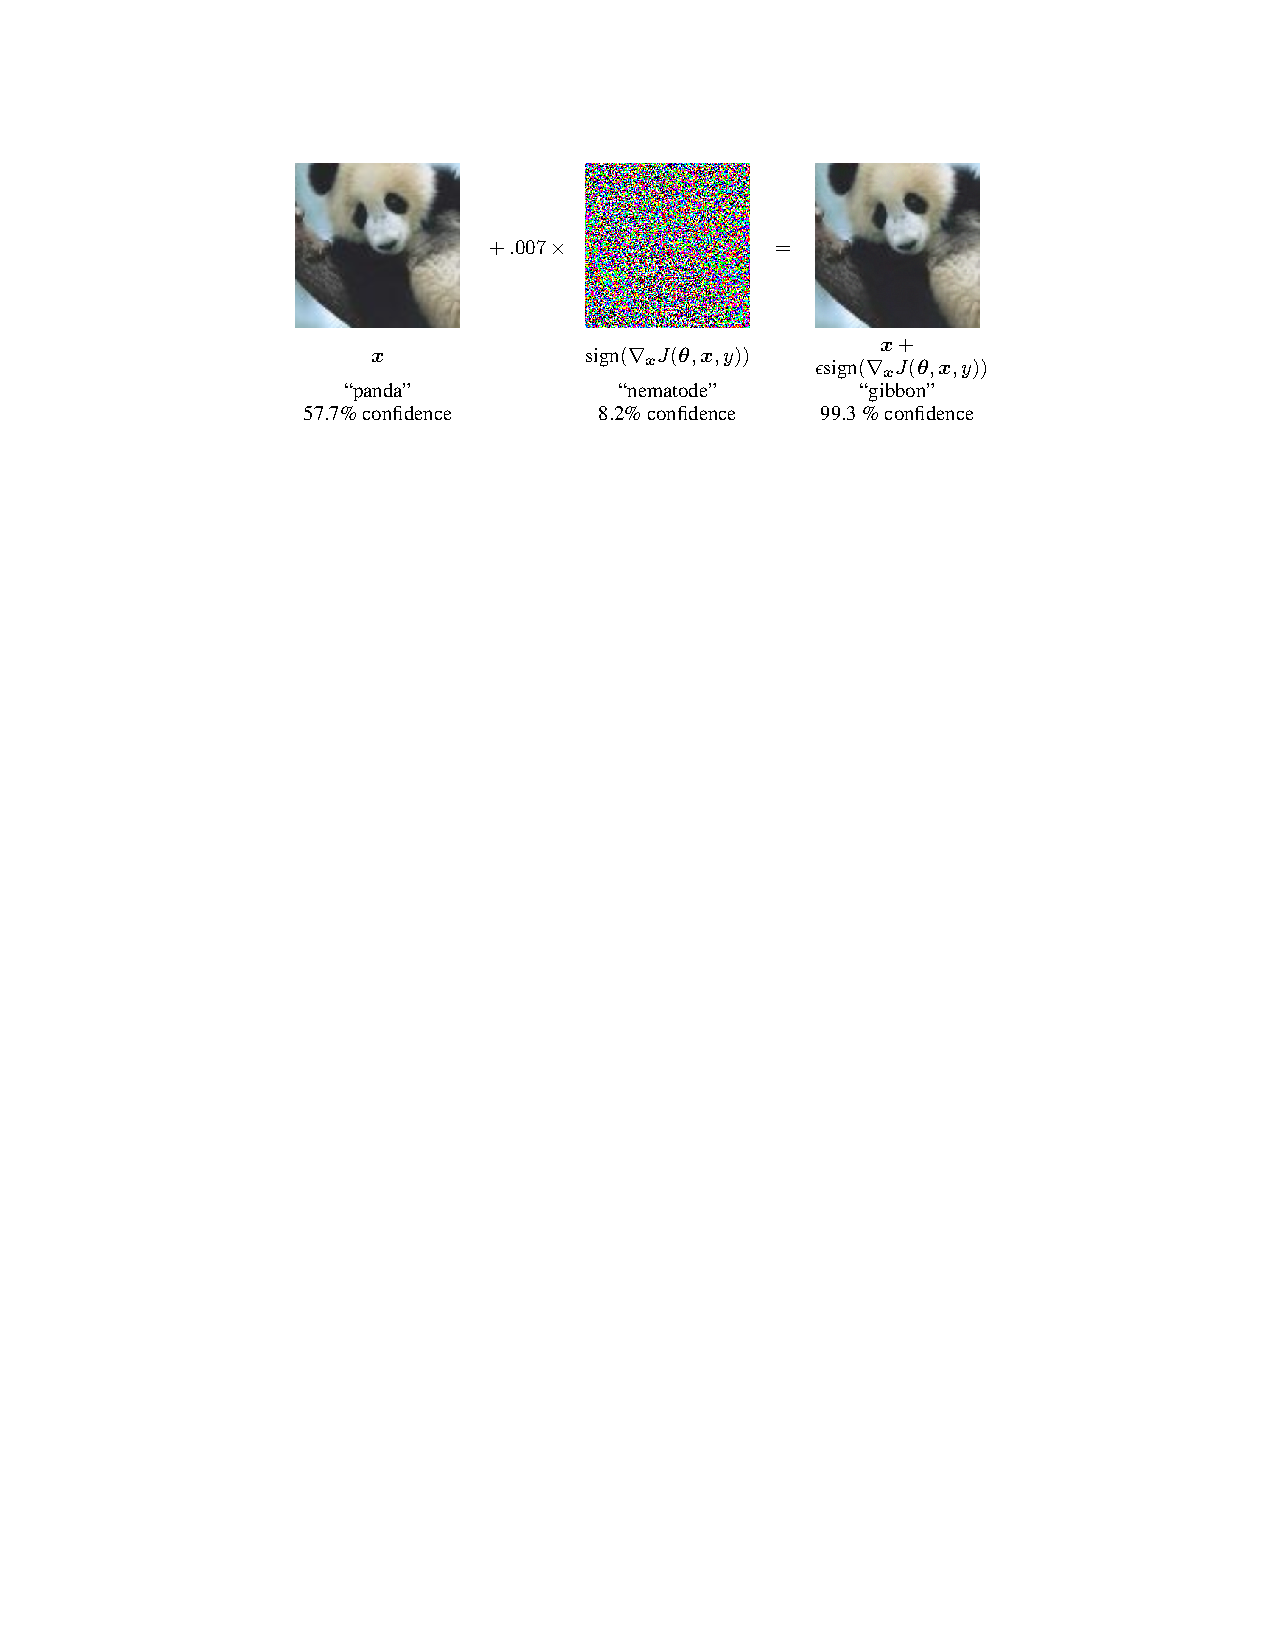
\includegraphics{fig/adversarial_example.pdf}
    \caption{对抗样本的一个演示,干净的样本能够被GoogLeNet\cite{szegedy2015going}正确识别成熊猫(Panda),而添加了不可察觉的扰动的对抗样本却被识别成了长臂猿(Gibbon)。左边:干净样本;中间:扰动;右边:对抗样本。}
    \label{fig:adversarial_example}
\end{figure}

在对抗样本的攻击下,深度神经网络表现出了非常差的鲁棒性,使得应用深度学习的系统都不可避免地存在着潜在的风险,尤其是在安全性非常重要的任务上。另一方面,深度神经网络如此反直觉的特性,让我们不得不反思:那些号称在某项任务上深度学习模型超越人类水平的标语真的有意义吗?那些深度网络的智能水平真的比得上人类智能吗?从对抗鲁棒性的语境下看,答案当然是否定的。对抗鲁棒性问题如此具有现实意义,同时又带有一定的哲学内涵,吸引了学者们前赴后继地进行研究,大量的防御方法被提出来,目的是为了能够让智能系统正确地认知对抗样本\cite{szegedy2013intriguing, gu2014towards, madry2018towards, papernot2016distillation, rozsa2016adversarial, zheng2016improving}。 然而,这些被提出来的防御措施大部分都不够有效,它们可以被更强大的敌人成功攻击\cite{carlini2017towards}。同时也有一些工作旨在验证和训练可证明鲁棒的神经网络,但是这些方法只能提供单点的保证,而且它们需要巨大的计算代价, 因此无法被推广到更为现实的数据集中\cite{raghunathan2018certified, pmlr-v80-wong18a, wong2018scaling}。 另外,基于检测的防御方法也被大量地提出来\cite{grosse2017statistical, gong2017adversarial, metzen2017detecting, li2017adversarial, feinman2017detecting},然而, Carlini 和 Wagner的研究\cite{carlini2017adversarial}表明这些防御措施都可以被使用具有针对性的攻击机制的敌人轻易地规避。

\begin{figure}[h]
    \centering
    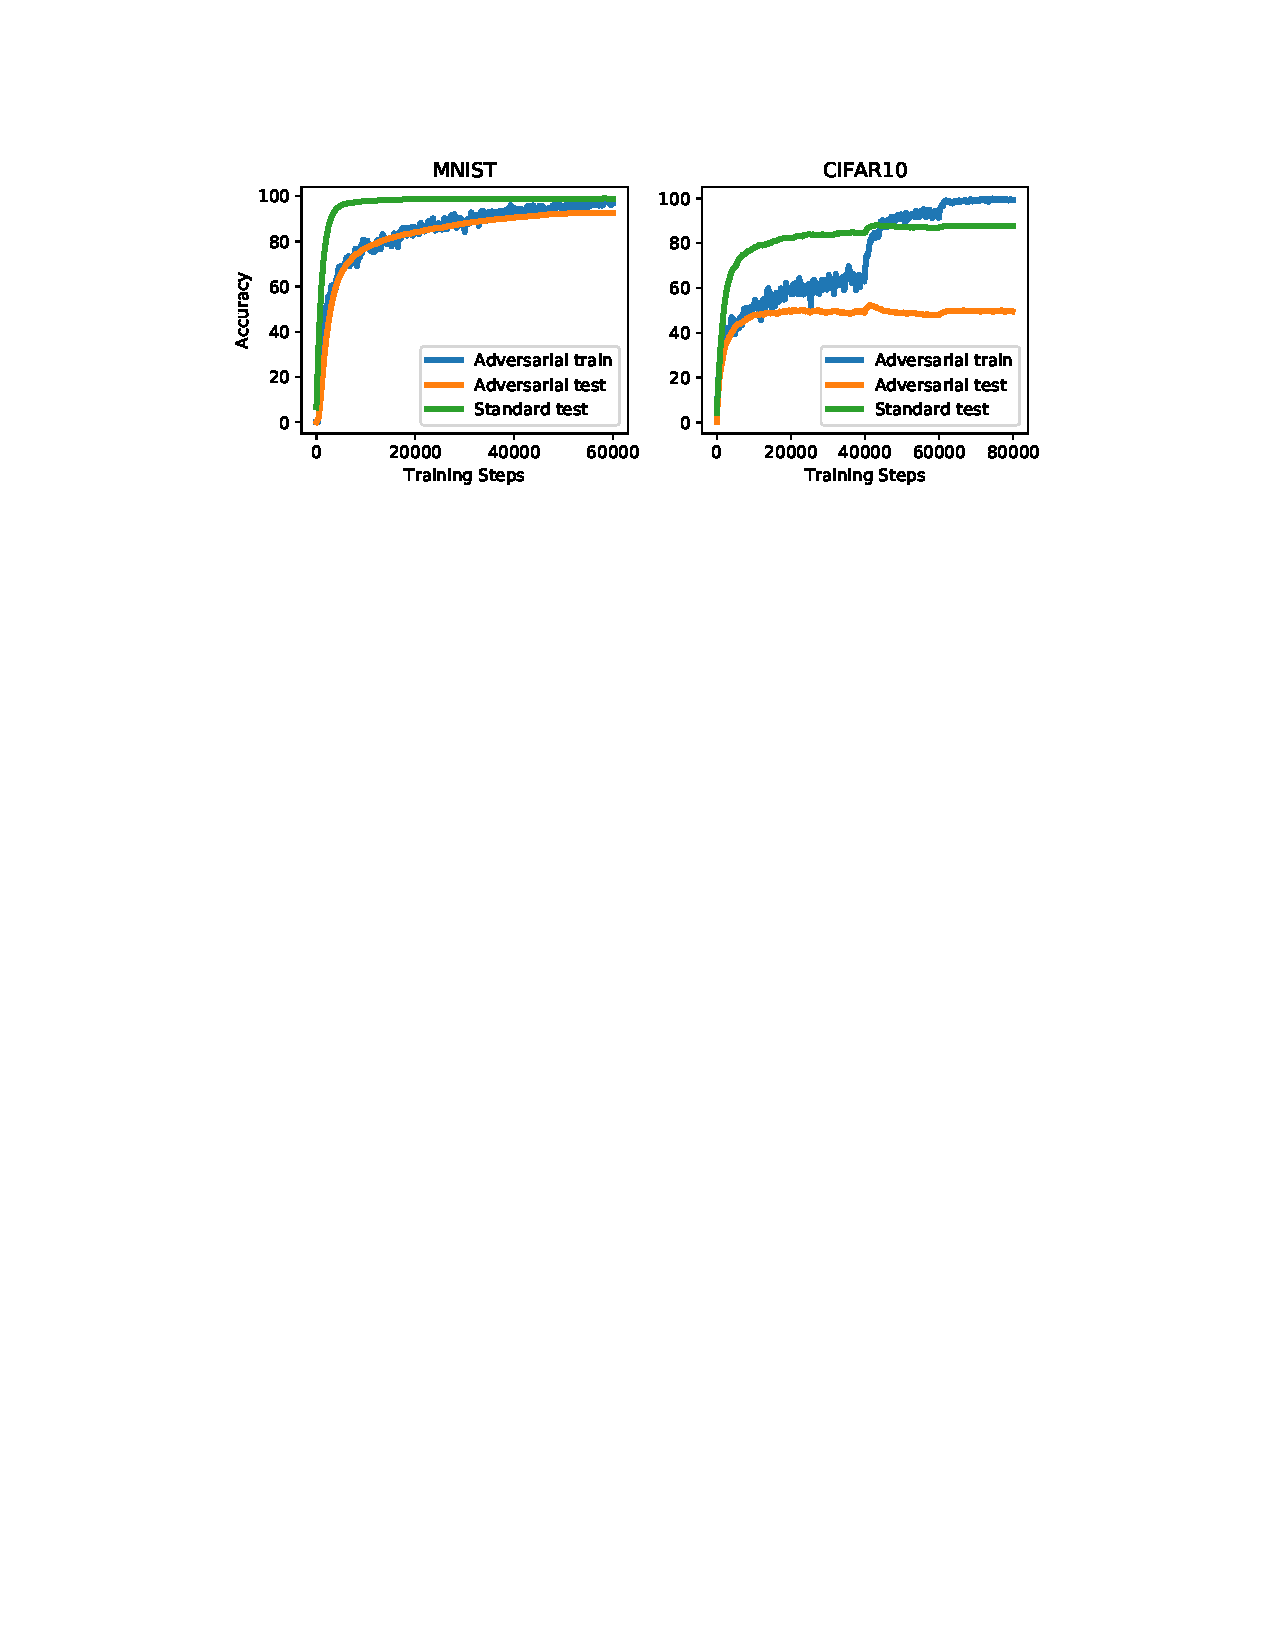
\includegraphics{fig/robust_optimization.pdf}
    \caption{在MNIST和CIFAR10上进行鲁棒优化(即对抗训练)的分类正确率}
    \label{fig:robust_optimization}
\end{figure}

许多的防御方法被提出来不久就被更强的攻击方法击败,唯有对抗训练(Adversarial training)这个简单且有效的方法经受住了时间的考验。对抗训练是将对抗样本作为训练集的一部分,让模型去学习,目的是使深度神经网络对未来(即测试时)样本的攻击具有更好的鲁棒性。Madry 等人\cite{madry2018towards}从鲁棒优化(Robust optimization) 的角度解释了对抗训练,表明对抗训练的过程是在每个训练样本的周围空间里寻找最坏的样本用以训练最优的分类器,并建议在对抗训练时使用一阶敌人(First-order adversary)作为自然且普适的安全性保证。

然而对抗训练本身的性能并不够理想。虽然通过合适的模型和适当的优化过程,对抗训练出来的模型可以将训练集样本较好地拟合,但是在测试集上的泛化性能却很差\cite{schmidt2018adversarially}。如\autoref{fig:robust_optimization}所示, 在 MNIST 上,对抗测试集精度接近对抗训练集精度(但还是有一些差距);在 CIFAR10 上,虽然模型在标准(非对抗)的测试集上有较高的精度,但在鲁棒精度上有一个非常大的鸿沟,即对抗测试集上的精度远低于对抗训练集上的精度。

对抗训练泛化能力的不足,暗示着我们应该为对抗训练设计更为有效的正则化方法,尤其是在深度神经网络过参数化的情况下。本文的主要任务,就是尝试结合度量学习的思想,利用相关的正则化方法,以提高对抗训练的泛化性能,并通过大量的实验进行有效性验证。
\chapter{国内外研究现状}

本章介绍与本文相关的三个主题:深度学习、度量学习、对抗样本问题。本文研究的是如何结合度量学习的思想以缓和深度学习中的对抗样本问题,我们针对的主要是比较基础的图像分类任务,其它任务中的对抗样本问题不在本文讨论范畴,但值得进一步推广和探索。

\section{深度学习}

2006年,多伦多大学教授Geoffrey Hinton及其学生Rusian发表在世界顶级学术期刊《科学》上的一篇论文引发了深度学习在研究领域和应用领域的发展热潮\cite{hinton2006reducing}。这篇文献提出了两个主要观点:(1)、多层人工神经网络有很强的特征学习能力,深度学习模型学习得到的特征数据对原数据有更本质的代表性,这将大大便于分类和可视化问题;(2)、对于深度神经网络难以训练的问题,可以采用逐层训练的方法解决。

深度学习发展到今天,已经在许多领域大放异彩,例如:计算机视觉、自然语言处理、医学影像分析、语音、游戏、图网络、时间序列、机器人控制、计算机编程等。本节主要介绍深度学习在图像分类(Image classification)和目标检测(Object detection)上的进展。

\subsection{图像分类}

早在1989年,受到生物学家Hubel和Wiesel的动物视觉模型\cite{hubel1962receptive}的启发,Yann LeCun等人就提出了一个多层的卷积神经网络(Convolutional Neural Network, CNN)\cite{lecun1989backpropagation}。但由于优化方法、数据量和计算能力等限制,直到2012年,Hinton等人才采用更深的卷积神经网络模型AlexNet在著名的ImageNet问题上取得当时世界上最好的成果,使得对于图像识别的研究工作前进了一大步\cite{krizhevsky2012imagenet}。

\begin{figure}[h]
    \centering
    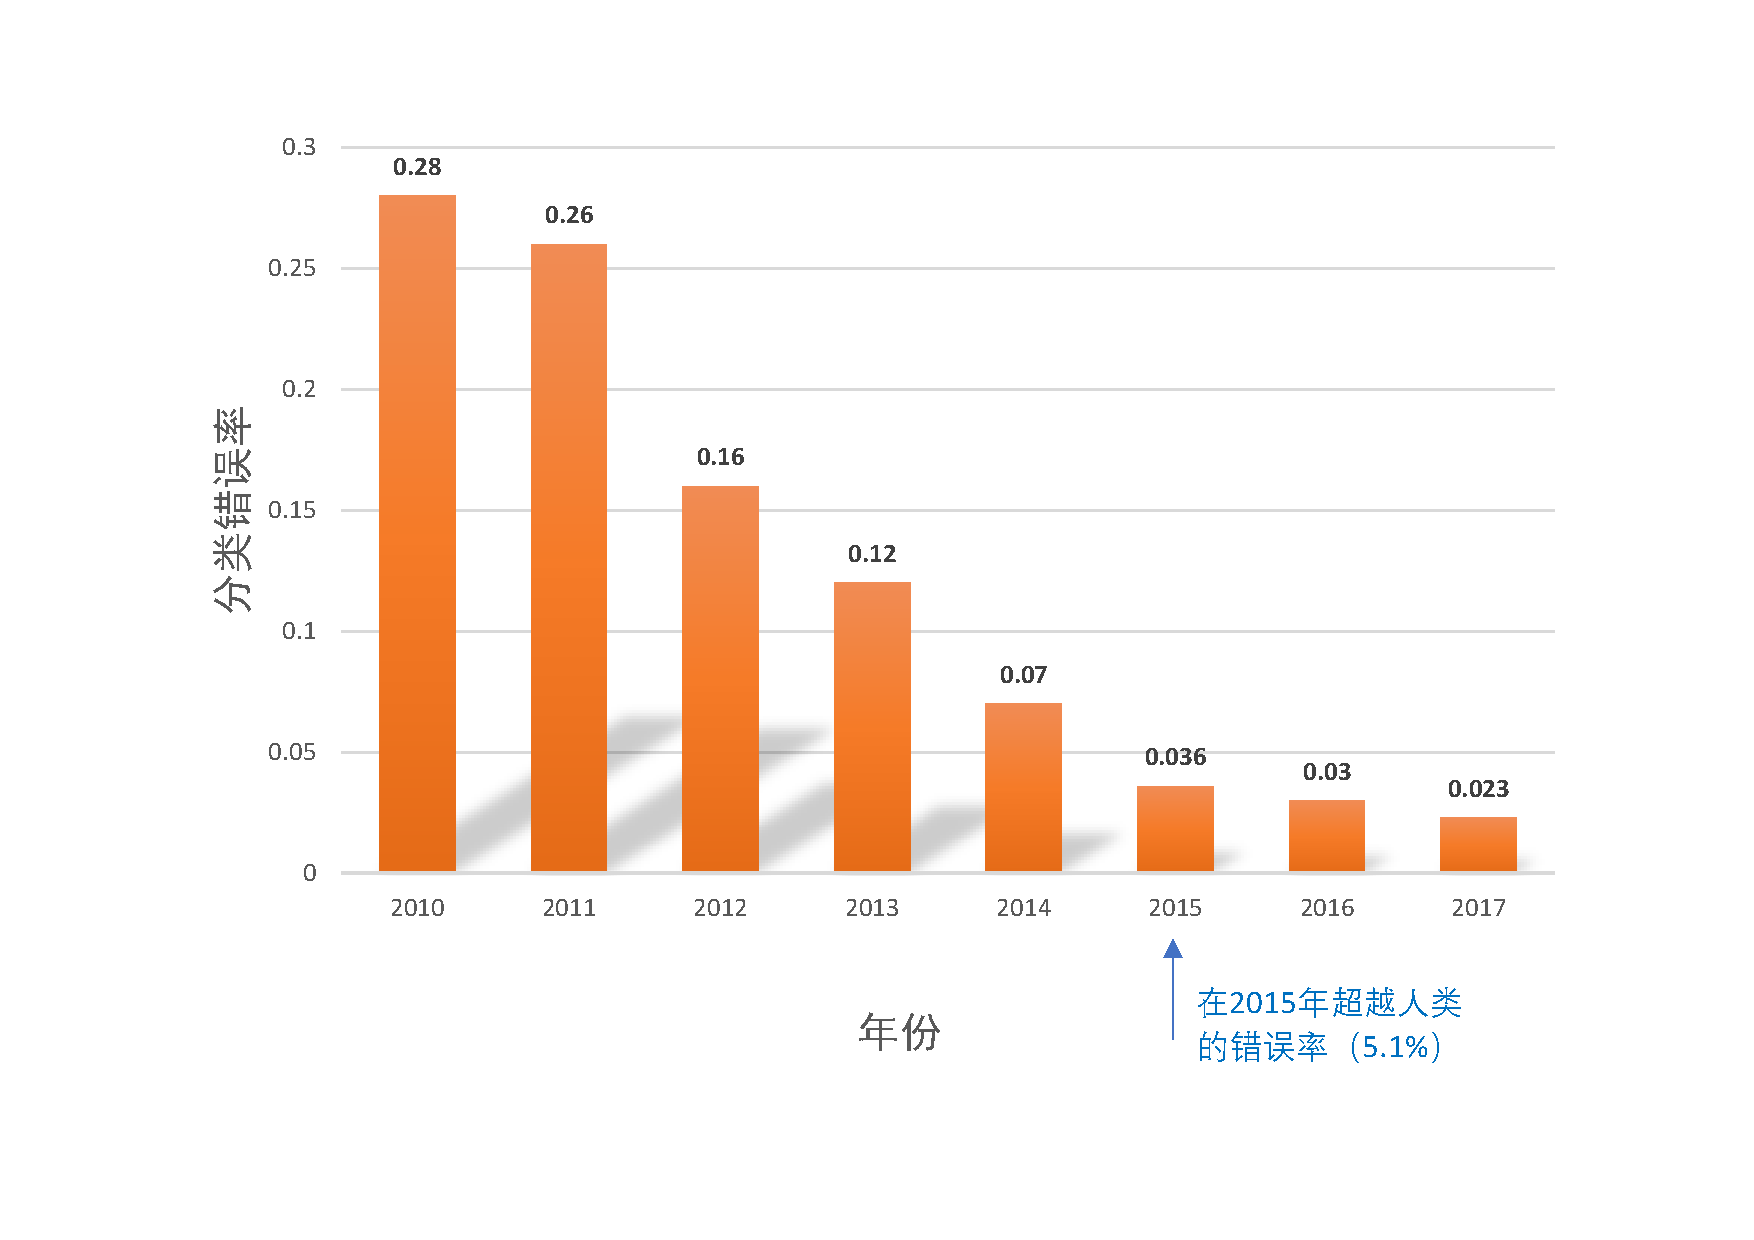
\includegraphics[width=15cm]{fig/imagenet.pdf}
    \caption{2010 $\sim$ 2017年ImageNet分类任务错误率}
    \label{fig:imagenet}
\end{figure}

2014年,更深的深度网络VGGNet\cite{simonyan2014very}和GoogLeNet\cite{szegedy2015going}被成功训练,分别为16层和22层。2015年,He等人提出ResNet\cite{he2016deep},利用残差单元(Residual unit)有效地缓和了梯度消失问题,成功训练了一个152层的深度神经网络,进一步提高了在ImageNet上的分类性能。2017年,注意力机制被引入深度网络架构中,Hu等人提出SENet\cite{hu2018squeeze},利用通道间的自注意力机制,赢得了最后一届ImageNet竞赛的冠军。随后Woo等人提出CBAM模块\cite{woo2018cbam},结合通道间和空间的自注意力,进一步提升了性能。\autoref{fig:imagenet}展示了2010 $\sim$ 2017年ImageNet分类错误率变化情况,从错误率的指标上看,深度网络已经超越人类。

\subsection{目标检测}

自从AlexNet获得ILSVRC 2012挑战赛冠军后,用CNN进行分类成为主流。2014年,Girshick等人提出R-CNN\cite{girshick2014rich},利用候选区域方法(Region proposal method)创建目标检测感兴趣的区域(Resion of Interest, ROI),再送入CNN进行分类,此方法每预测一张图片需要49秒。2015年,Ross Girshick提出Fast R-CNN\cite{girshick2015fast},利用特征图代替原图生成ROI,显著地减少处理时间至每张图片2.3秒。2016年,Ren等人提出Faster R-CNN\cite{ren2015faster},使用内部的候选区域网络代替了外部的候选区域方法,使得ROI的生成效率进一步提高,每张图片的处理时间减小到0.2秒。

以上的目标检测器由于候选区提取和分类是分开做的,被称为二次检测器(Two-stage detector),与之对应的是随后提出的单次检测器(One-stage detector)。Liu等人提出的SSD模型\cite{liu2016ssd}和Redmon等人提出的YOLO模型\cite{redmon2016you, redmon2017yolo9000, redmon2018yolov3}将候选区提取和分类用端到端(End-to-end)的方式融合到一起训练,使得目标检测器真正达到了实时检测的程度,但对小目标的检测效果较差。Lin等人提出特征金字塔网络(Feature Pyramid Network, FPN)\cite{lin2017feature},利用多尺度特征图提高准确率。

\section{度量学习}

过去的十几年里,大量的度量学习(Metric Learning)算法被提出,其中最典型的是对比损失(Contrastive loss)\cite{chopra2005learning, hadsell2006dimensionality}和三元组损失(Triplet loss)\cite{weinberger2009distance, chechik2010large}。它们的目标通常是学习一个良好的距离度量,使得正样本对(Positive pair)之间的距离尽量小,负样本对(Negative pair)之间的距离尽量大。这些度量学习方法被提出时,只能够学习一个线性变换,无法很好地刻画现实数据中的非线性流形结构。为了解决这个问题,核技巧通常被采用,先将样本映射到一个高维的特征空间中,然后再在这个高维空间里学习一个距离度量\cite{tsang2003distance, yeung2007kernel}。然而,这些方法无法显式地得到一个非线性映射函数,因此无法被应用到更大规模的数据上。

自深度学习表现出强大的表示学习能力之后,深度神经网络便被引入到度量学习之中,以学习一个非线性映射。Hu等人将深度网络应用到对比损失中\cite{hu2014discriminative},Hoffer等人将深度网络应用到三元组损失中\cite{hoffer2015deep}。然而,将深度网络直接地应用到度量学习中,带来的问题是:这些方法随机采样样本对或三元组以构成训练批次,无法在小批次随机梯度下降的训练过程中充分利用一批次里的所有训练样本。Kihyuk和Oh Song等人分别提出一种新颖的采样方式\cite{oh2016deep, sohn2016improved},能够充分利用小批次里的所有样本,提升了深度度量学习(Deep Metric Learning)的性能。

\section{对抗样本问题}

早在十几年前,对抗样本问题就在传统机器学习中被讨论过。2004年,Dalvi等人首次讨论了对抗样本,把这个问题看做敌人和分类器之间的一个博弈问题\cite{dalvi2004adversarial},在对抗样本上的攻击和防御变成了一场迭代式的博弈。通过增加字符以避免检测,对抗攻击曾被应用到垃圾邮件过滤系统中\cite{dalvi2004adversarial, biggio2010multiple}。2013年,Biggio等人首先提出一个基于梯度的方法生成对抗样本以攻击浅层的分类器,比如支持向量机、一个两层的神经网络\cite{biggio2013evasion}。与深度学习中的对抗样本相比,传统机器学习中的方法在修改数据上拥有更大的自由度,第一个被用来评估攻击方法的数据集是MNIST,但此时生成的对抗样本能被人类轻易地分辨出来。

在传统机器学习中,攻击和防御方法都在特征提取过程中下了很大功夫,甚至可以影响数据采集过程,在对人类的影响上并没有太多的考虑\cite{roli2013pattern};而在深度学习中,只需要关心原始数据的输入,且非常强调对人类视觉系统的影响。

本文重点研究图像分类任务中的对抗样本:使用一个第三方发布的预训练的分类器,用户输入一张图片以得到分类器的预测结果。对抗样本是在干净的原始样本上添加一些微小的扰动,这些扰动通常无法被人类感知到。然而,这样的扰动可以误导图片分类器,用户将得到一个不正确的预测结果。记$f$为一个训练好的深度学习模型,$x$为一个原始的输入样本数据,一个对抗样本$x'$的生成过程可以被描述为一个带约束的优化问题:
\begin{equation}
    \begin{aligned}
    \min_{x^{\prime}} \quad & \left\|x^{\prime}-x\right\| \\
    s.t. \quad & f\left(x^{\prime}\right)=l^{\prime}, \\ 
               & f(x)=l, \\ 
               & l \neq l^{\prime}, \\ 
               & x^{\prime} \in[0,1],
\end{aligned}
\end{equation}
其中$l$和$l'$表示$x$和$x'$的输出标记,$\|\cdot\|$表示两个样本点之间的距离,$\eta=x'-x$表示添加在$x$上的扰动。这个优化问题在输入数据有范围限制的情况下,误导模型预测结果的同时最小化扰动。

\subsection{攻击方法}

2014年,Szegedy等人首先提出了针对深度神经网络的对抗样本,提出了一种名为L-BFGS的攻击方法。L-BFGS方法使用代价较高的线性搜索方法去寻找参数的最优值,这非常耗时且实用性不强,因此Goodfellow等人提出了一个快速的生成对抗样本的方法,称作快速梯度符号方法(Fast Gradient Sign Method, FGSM),此方法仅仅只需要沿着每个像素的梯度符号方向执行一步梯度更新,便可生成如\autoref{fig:adversarial_example}所示的对抗样本\cite{goodfellow2014explaining}。2016年,Kurakin等人为了将对抗样本应用到物理世界中,他们扩展了FGSM方法,使用更细化的优化过程和多次的迭代以生成更具有迁移能力的对抗样本,称作基本迭代方法(Basic Iterative Method, BIM),成功欺骗了一个运行在手机上的ImageNet分类器\cite{kurakin2016adversarial}。Moosavi-Dezfooli等人提出DeepFool方法以寻找与原始样本距离最小的对抗样本\cite{moosavi2016deepfool}。2017年,Carlini和Wagner提出了一个非常强大的攻击方法C\&W's Attack,使得许多防御方法失效\cite{carlini2017towards}。Chen等人提出一种基于零阶优化(Zeroth Order Optimization, ZOO)的攻击方法,这个方法不需要梯度信息,所以可以被直接应用到黑盒攻击上,无需迁移\cite{chen2017zoo}。Moosavi-Dezfooli等人基于DeepFool提出了一种普适性的对抗攻击(Universal adversarial attack),能够找到攻击尽量多样本的一个普适性的扰动。为了让人类无法察觉对抗扰动,Su等人提出单像素攻击(One pixel attack),利用进化算法寻找一个像素点进行扰动\cite{su2019one}。

在视觉应用方面。2016年,Sharif等人设计了一个眼镜形状的对抗扰动,以攻击基于深度神经网络的人脸识别系统\cite{sharif2016accessorize}。2017年,Xie等人提出密集敌人生成(Dense Adversary Generation, DAG)算法,能够生成针对目标检测和语义分割系统的对抗样本\cite{xie2017adversarial}。2019年,腾讯科恩实验室对特斯拉Autopilot自动驾驶系统的安全性进行研究,成功攻击了Autopilot系统的外部天机状况识别系统和道路交通标线识别系统,分别使得车辆雨刷误启动和驶入反向车道\cite{tecent2019tesla}。

在自然语言处理应用方面。2017年,针对阅读理解系统,为了产生与正确答案一致且不混淆人的对抗性例子,Jia等人在段落末尾增加了对抗性字段\cite{jia2017adversarial}。2019年,针对语音识别系统,Qin等人提出了一种有效的人类不可察觉的音频对抗样本生成方法,此方法充分利用了听觉掩模的心理声学原理,对任意的全语句目标都达到了百分之百的攻击成功率,进一步,他们发现在物理世界中通过空气传播此对抗音频后,攻击仍然有效\cite{qin2019imperceptible}。

\subsection{防御方法}

2016年,Papernot等人提出使用网络蒸馏(Network distillation)作为一个防御对抗样本的手段\cite{papernot2016distillation},但随后被Carlini等人提出的C\&W's Attack成功击破。2017年,许多检测方法被用来检测对抗样本。有的工作提出使用一个基于深度网络的二元分类器用于检测并过滤对抗样本\cite{lu2017safetynet, metzen2017detecting, gong2017adversarial},有的工作提出添加一个离群类到原始的深度学习模型中以检测并过滤对抗样本\cite{grosse2017statistical},还有的工作发现对抗样本的分布与干净样本的不同,提出用基于PixelCNN\cite{Salimans2017pixelcnn}排序的p值进行对抗样本的检测和拒绝\cite{song2017pixeldefend}。然而,Carlini和Wagner总结了以上对抗性的检测方法,展示了这些检测防御方法都可以被更具有针对性的攻击轻易规避\cite{carlini2017adversarial, carlini2017magnet}。2018年,许多梯度掩码(Gradient masking)的方法被提出用来增强深度网络的鲁棒性。Jacob等人提出用温度计编码(Thermometer encoding)来提高鲁棒性\cite{buckman2018thermometer};Guo等人提出将输入的图片进行五个预变换,以消除对抗扰动,提升模型鲁棒性\cite{guo2018countering};Dhillon等人提出随机激活剪枝(Stochastic Activation Pruning, SAP),随机抛弃部分神经元以消除对抗扰动的影响\cite{s.2018stochastic};Xie等人提出在输入样本被送入模型前对样本进行随机变换,以消除对抗扰动的影响\cite{xie2018mitigating};Song等人提出使用PixelCNN模型将潜在的对抗样本投影到真实的数据流形上以消除对抗扰动\cite{song2018pixeldefend};Samangouei等人提出使用生成对抗网络将样本投影到生成器的数据流形中以消除对抗扰动\cite{samangouei2018defensegan};然而,以上所有梯度掩码的方法都被Athalye等人使用具有针对性的攻击方法一一破解\cite{pmlr-v80-athalye18a}。

同时,Athalye等人也指出,目前只有对抗训练这一种防御方式无法被完全击破,但对抗训练也有自身的问题\cite{pmlr-v80-athalye18a}。虽然对抗训练在MNIST上的鲁棒性比较令人满意\cite{madry2018towards},但在ImageNet这样的数据集上的鲁棒性就差强人意了\cite{kurakin2017adversarial}。而且对抗训练在CIFAR10和ImageNet上的泛化性能比较差,这个泛化性能包括在测试时对同一种攻击方式(与训练时使用的攻击方式相同)的鲁棒性和测试时对其它攻击方式(与训练时使用的攻击方式不同)的鲁棒性,通常认为对抗训练的样本复杂度远高于自然训练的样本复杂度\cite{schmidt2018adversarially}。

为了提高对抗训练的泛化能力,Kannan等人提出对抗逻辑配对(Adversarial Logit Pairing),提高了对抗训练在ImageNet上的泛化能力\cite{kannan2018adversarial},并被NIPS 2018接收,但随后被人指出并实验上证明了该方法并没有真正地提在ImageNet上的泛化能力\cite{engstrom2018evaluating},于是ALP又被作者从NIPS上撤稿。本文也对ALP的有效性进行了一些探究,详见章节\ref{section:generalization}。Song等人提出使用将干净样本分类和对抗样本分类看做一个域适应的问题,采用最大均值散度(Maximum Mean Discrepancy, MMD)和相关性匹配(CORrelation ALignment, CORAL)作为正则化项提高对抗训练的泛化能力\cite{song2018improving}。Farnia等人提出使用谱归一化来提高对抗训练的泛化能力\cite{farnia2018generalizable}。
\chapter{对抗训练及其正则化方法}

本文专注于对基于深度学习的模型的攻击和防御,我们假设对手仅仅能够在模型的测试阶段实施攻击,对手只能在模型训练之后篡改模型的输入数据。已训练的模型和训练集数据均不可被篡改,但对手拥有已训练的模型的所有知识(模型架构和参数),这是符合目前大部分在线机器学习服务系统现状的假设。本节先介绍与对抗训练相关的几个攻击方法,再讨论对抗训练的泛化能力,最后介绍并提出相关的正则化方法。

\section{攻击方法}

本小节介绍三种攻击方法:快速梯度符号方法(Fast Gradient Sign Method, FGSM)\cite{goodfellow2014explaining}、投影梯度下降(Projected Gradient Descent, PGD)\cite{madry2018towards}、Carlini和Wagner的攻击(C\&W's Attack)\cite{carlini2017towards}。

记干净样本集合为$\mathcal{D}$,对抗样本集合为$\mathcal{A}$。我们有一个基于神经网络的分类器$f(x) : \mathbb{R}^d \to \mathbb{R}^k$,对每一个输入$x \in [0, 1]^d$,$f(x)$输出对应的概率分布,$k$表示分类任务的类别总数。令$\varphi$表示从输入层到逻辑层(在最后一个softmax函数之前的一层)的映射,于是$f(x) = softmax(\varphi(x))$。记$\epsilon$为扰动的幅度,记$x^{adv}$为对抗样本,它是由原始样本$x$受到扰动而得到的。图片分类的损失函数记为$J(x, y)$。

\subsection{FGSM}

Goodfellow等人介绍了用FGSM生成对抗样本,通过在梯度的方向上添加扰动。
\begin{equation}
    x^{a d v}=x+\epsilon \cdot \operatorname{sign}\left(\nabla_{x} J\left(x, y_{t r u e}\right)\right)
\end{equation}
与其它方法比起来,FGSM是一个简单、快速且有效的敌人,因此FGSM非常适合用于对抗训练。

\subsection{PGD}

PGD是Madry等人介绍的一种攻击方式,是FGSM的迭代变种。此方法迭代地执行$k$次FGSM,每次的步长为$\alpha$。
\begin{equation}
    \begin{aligned}
        x^{a d v_{0}} & =x \\
        x^{a d v_{t+1}} & =x^{a d v_{t}}+\alpha \cdot \operatorname{sign}\left(\nabla_{x} J\left(x^{a d v_{t}}, y_{t r u e}\right)\right. \\
        x^{a d v_{t+1}} & =\operatorname{\textbf{clip}}\left(x^{a d v_{t+1}}, x^{a d v_{t+1}}-\epsilon, x^{a d v_{t+1}}+\epsilon\right) \\ 
        x^{a d v} & =x^{a d v_{k}}
    \end{aligned}
\end{equation}
这里$\textbf{clip}(\cdot, a, b)$函数的功能是将它的输入裁剪到$[a, b]$范围内。在白盒攻击下,PGD通常拥有比FGSM更高的攻击成功率。

\subsection{C\&W's Attack}

C\&W's Attack是Carlini和Wagner提出用来攻击防御性蒸馏(Defensive distillation)\cite{papernot2016distillation}的一种强大的攻击方法。对抗扰动$\delta$通过以下的优化过程得到:
\begin{equation}
    \begin{aligned}
        {\min_{\boldsymbol{\delta} \in \mathbb{R}^{n}}} \quad & {\|\boldsymbol{\delta}\|_{p}+c \cdot f(\mathbf{x}+\boldsymbol{\delta})} \\
        {\text { s.t. }} \quad & {\mathbf{x}+\boldsymbol{\delta} \in[0,1]^{n}}
    \end{aligned}
\end{equation}
其中$c>0$是一个合适的常数,$\ell_{2}$、$\ell_{0}$ 和 $\ell_{\infty}$范数都可以考虑。

\section{对抗训练}

在本文研究的分类任务中,我们将模型的泛化能力细分为两种:
\begin{enumerate}
    \item 标准泛化能力(Standard generalization),即表示为模型在标准的测试集(不含对抗样本)上的分类准确率。
    \item 鲁棒泛化能力(Robust generalization),即表示为模型在对抗的测试集(不含干净样本)上的分类准确率。
\end{enumerate}

防御深度模型的一个非常直觉的方式是对抗训练,它在模型训练过程中向训练集里注入对抗样本。Goodfellow等人首次提出向模型同时送入原始样本和用FGSM生成的对抗样本以增加鲁棒性\cite{goodfellow2014explaining},目标函数为:
\begin{equation}
    \hat{J}\left(x, y_{t r u e}\right)=\alpha J\left(x, y_{t r u e}\right)+(1-\alpha) J\left(x+\epsilon \operatorname{sign}\left(\nabla_{x} J\left(x, y_{t r u e}\right), y_{t r u e}\right)\right.
\end{equation}
Kurakin等人在ImageNet上实现了对抗训练,发现了标签泄露(Label leaking)效应,并建议在对抗训练过程中不要使用基于真实标签$y_{true}$的FGSM方法,而应该使用基于最大可能标签的FGSM方法\cite{kurakin2017adversarial},本文的所有实验中对抗训练过程便采用了避免标签泄露的FGSM方法。其它的一些方法在对抗训练过程中使用PGD方法或更加复杂的优化方法产生最坏情况的对抗样本,然而这样的方式时间复杂度过高,导致推广到更大规模的神经网络上非常困难\cite{madry2018towards, pmlr-v80-wong18a}。

以上所有的对抗训练方法都会存在鲁棒泛化能力不佳的问题。本文考虑的是在对抗训练过程中用最简单的FGSM方法产生对抗样本,但使用额外的正则化项以提高鲁棒泛化能力,这样的好处是不需要在生成对抗样本的优化过程花费太多时间,更容易拓展到更大规模的数据集和模型上。

\section{对抗训练中的正则化方法}

深度学习中对抗样本的存在性是一个反直觉的特性,一个被普遍接受的解释是:对抗样本是模型的内在的盲点区域,这个盲区的结构与数据分布紧密相关,以一种不那么明显的方式\cite{szegedy2013intriguing}。这种不明显体现在,对抗样本和干净样本在我们人类看来区别并没有那么地明显,甚至不可察觉,但事实上,对于模型来说,这种不明显的区别是致命的。这种致命体现在,两个在原始特征空间中非常邻近的样本点,经过深度网络一系列非线性变换后,两个样本点在隐空间中的距离竟然会变得很远,以至于最终落在了模型的两个不同的判决区域。

一个直觉的方案是在隐空间中尽量拉近对抗样本与干净样本的距离,期望使得模型不再将两个样本点(对抗样本和原始样本)判为不同类别。这个思想就是度量学习中的对比损失,学习一个良好的深度网络,使得在隐空间中对抗样本和干净样本之间的距离尽量小。

对比损失可以形式化为:
\begin{equation}
    L
    = 
    \frac{1}{(|\mathcal{D}| + |\mathcal{A}|)^2} \sum_{x_i, x_j \in \mathcal{D} \cup \mathcal{A}} w_{ij}\big\|\varphi(x_i) - \varphi(x_j)\big\|_2^2
    \ ,
    \label{contrastive_loss}
\end{equation}
其中$w_{ij}$定义为:
\begin{equation}
    w_{ij} = \left\{
    \begin{array}{rl}
    1  & \quad \textnormal{if } (x_i, x_j) \in \mathcal{P}_{sim} \ ,\\
    -1 & \quad \textnormal{if } (x_i, x_j) \in \mathcal{P}_{dis} \ ,\\
    0  & \quad otherwise \ .
    \end{array} \right.
    \label{metric_weight}
\end{equation}
其中$\mathcal{P}_{sim}$表示相似样本对集合,$\mathcal{P}_{dis}$表示不相似样本对集合。这里的式\eqref{contrastive_loss}在度量学习中只是一个最基本的形式,本文这样写是为了阐明本文思路,对比损失的其它变体形式在这里不予赘述。

为了将对比损失的思想作为一个正则化项,合适地融入对抗训练的损失中,下面介绍三种构造方式:对抗逻辑配对(Adversarial Logit Pairing, ALP)\cite{kannan2018adversarial}、结合域适应的对抗训练(Adversarial Training with Domain Adaption, ATDA)\cite{song2018improving}、对抗流形正则化(Adversarial Manifold Regularization, AMR)。

\subsection{ALP} \label{section:alp}

ALP可以定义为:
\begin{equation}
    L_{alp}
    = 
    \frac{1}{|\mathcal{D}|} \sum_{x_i \in \mathcal{D}} \big\|\varphi(x_i) - \varphi(x_i^{adv})\big\|_2^2 \ ,
    \label{alp}
\end{equation}
其中$x_i^{adv}$是$x_i$对应的使用FGSM攻击方法生成的对抗样本。式\eqref{alp}旨在缩小每个样本点和它对应的对抗样本点间的欧式距离,即在式\eqref{metric_weight}中,$\mathcal{P}_{sim} = \{(x_i, x_i^{adv}) | x_i \in \mathcal{D} \}$,$\mathcal{P}_{dis} = \varnothing$。

Kannan等人在提出ALP的文章中,他们仅仅在ImageNet上进行了有效性验证,在FGSM攻击的对抗训练过程中增加ALP正则化项,发现这样训练的模型对FGSM敌人和PGD敌人的鲁棒泛化能力都得到了提高\cite{kannan2018adversarial},随后却被人发现通过简单的增加PGD攻击的迭代次数便可将PGD鲁棒精度降为0.6\%\cite{engstrom2018evaluating},这篇文章因此从NIPS 2018撤稿。本文将在MNIST、SVHN等数据集上对ALP的有效性进行验证,并画出PGD鲁棒精度随迭代次数增多而下降的收敛曲线,以保证结论的准确性,详见章节\ref{section:convergence}。

\subsection{ADTA}

把对抗样本和干净样本看成两个不同的域,结合域适应的思想,ATDA提出用最大均值散度(Maximum Mean Discrepancy, MMD)\cite{borgwardt2006integrating}和相关性匹配(CORrelation ALignment, CORAL)\cite{sun2016deep}作为正则化项提高对抗训练的泛化能力\cite{song2018improving}。这和对比损失中点到点的拉近目标是有所区别的,MMD和CORAL是一种集合到集合的拉近。

MMD的目标是最小化干净样本和对抗样本的均值向量间的距离:
\begin{equation}
    L_{mmd} 
    = 
    \frac{1}{k} \Big\| \frac{1}{|\mathcal{D}|} \sum_{x\in\mathcal{D}}F(x_i) - \frac{1}{|\mathcal{A}|} \sum_{x^{adv}\in\mathcal{A}}F(x_i^{adv}) \Big\|_1 
    .
\end{equation}

CORAL的目标是最小化干净样本和对抗样本间的协方差矩阵间的距离:
\begin{equation}
    L_{coral} 
    = 
    \frac{1}{k^2} \Big\| C_{\varphi(\mathcal{D})} -  C_{\varphi(\mathcal{A})} \Big\|_{\ell_1} 
    ,
\end{equation}
其中$C_{\varphi(\mathcal{D})}$和$C_{\varphi(\mathcal{A})}$分别是干净样本和对抗样本在逻辑空间(Logit sapce)上的协方差矩阵,$\| \cdot \|_{\ell_1}$表示矩阵的$L_1$范数。

\subsection{AMR}

流形正则化(Manifold Regularization, MR)在早期被提出,主要是希望通过这种方式去利用大量的未标记样本,来提高分类或回归任务的性能。它的主要思想是利用数据集的几何性状去对模型空间产生约束。该正则化项可以被估计为\cite{belkin2006manifold}:
\begin{equation}
    L_{mr}
    = 
    \frac{1}{|\mathcal{D}|^2} \sum_{x_i, x_j \in \mathcal{D}} w_{ij}\big\|\varphi(x_i) - \varphi(x_j)\big\|_2^2
    \ ,
\end{equation}
其中$w_{ij}$定义为:
\begin{equation}
    w_{ij} = \left\{
    \begin{array}{rl}
    \exp \left(\frac{-\left\|x_i-x_j\right\|_2^2}{t}\right)  & \quad \textnormal{if } (x_i, x_j) \in \mathcal{P}_{k} \ ,\\
    0  & \quad otherwise \ .
    \end{array} \right.
\end{equation}
其中温度参数$t \in \mathbb{R}$,$\mathcal{P}_{k}$表示集合$\mathcal{D}$中所有样本间的k近邻构成的样本对集合。该正则化项的直觉是:在原空间中非常接近的样本对,经过变换后,尽量在隐空间中也相近;在原空间不那么靠近的样本对,在隐空间中的紧密度也就不那么重要了(体现在$w_{ij}$的相对大小中)。

本文将流形正则化适应到对抗训练的环境中,提出对抗流形正则化(Adversarial Manifold Regularization, AMR),其主要思想是在原空间中非常接近的干净样本和对抗样本(k近邻),在隐空间中也应该尽量靠近。AMR可以被形式化为:
\begin{equation}
\begin{aligned}
    L_{amr}
    = \ &
    \frac{1}{|\mathcal{D}| \cdot |\mathcal{A}|} \sum_{x_i^{cln} \in \mathcal{D}} \sum_{x_j^{adv} \in \mathcal{A}} w_{ij}^{(1)} \big\|\varphi(x_i^{cln}) - \varphi(x_j^{adv})\big\|_2^2 \\
    + & 
    \frac{1}{|\mathcal{D}| \cdot |\mathcal{A}|} \sum_{x_i^{adv} \in \mathcal{A}} \sum_{x_j^{cln} \in \mathcal{D}} w_{ij}^{(2)} \big\|\varphi(x_i^{adv}) - \varphi(x_j^{cln})\big\|_2^2
    \ ,
\end{aligned}
\end{equation}
其中$w_{ij}^{(l)}(l\in\{1, 2\})$定义为:
\begin{equation}
    w_{ij}^{(l)} = \left\{
    \begin{array}{rl}
    \exp \left(\frac{-\left\|\varPhi(x_i)-\varPhi(x_j)\right\|_2^2}{t}\right)  & \quad \textnormal{if } (x_i, x_j) \in \mathcal{P}_{k}^{(l)} \ ,\\
    0  & \quad otherwise \ .
    \end{array} \right.
\end{equation}
其中温度参数$t \in \mathbb{R}$,$\mathcal{P}_{k}^{(1)}$表示集合$\mathcal{D}$中所有样本在集合$\mathcal{A}$中的k近邻构成的样本对集合,$\mathcal{P}_{k}^{(2)}$表示集合$\mathcal{A}$中所有样本在集合$\mathcal{D}$中的k近邻构成的样本对集合。$\varPhi(\cdot)$是一个特征提取器(自编码器、自然训练的分类器或对抗训练的分类器),之所以使用一个特征提取器来计算k近邻的距离,是因为在高维的图像数据中欧式距离已失效。
% \chapter{对抗训练的泛化能力}

本文专注于对基于深度学习的模型的攻击和防御,我们假设对手仅仅能够在模型的测试阶段实施攻击,对手只能在模型训练之后篡改模型的输入数据。已训练的模型和训练集数据均不可被篡改,但对手拥有已训练的模型的所有知识(模型架构和参数),这是符合目前大部分在线机器学习服务系统现状的假设。本节先介绍与本文相关的几个攻击方法,再讨论对抗训练的泛化能力。

\section{记号}

记干净样本集合为$\mathcal{D}$,对抗样本集合为$\mathcal{A}$。我们有一个基于神经网络的分类器$f(x) : \mathbb{R}^d \to \mathbb{R}^k$,对每一个输入$x \in [0, 1]^d$,$f(x)$输出对应的概率分布,$k$表示分类任务的类别总数。令$\varphi$表示从输入层到逻辑层(在最后一个softmax函数之前的一层)的映射,于是$f(x) = softmax(\varphi(x))$。记$\epsilon$为扰动的幅度,记$x^{adv}$为对抗样本,它是由原始样本$x$受到扰动而得到的。图片分类的损失函数记为$J(x, y)$。

\section{攻击方法}

本小节介绍三种攻击方法:快速梯度符号方法(Fast Gradient Sign Method, FGSM)\cite{goodfellow2014explaining}、投影梯度下降(Projected Gradient Descent, PGD)\cite{madry2018towards}、Carlini和Wagner的攻击(C\&W's Attack)\cite{carlini2017towards}。

\subsection{FGSM}

Goodfellow等人介绍了用FGSM生成对抗样本,通过在梯度的方向上添加扰动。
\begin{equation}
    x^{a d v}=x+\epsilon \cdot \operatorname{sign}\left(\nabla_{x} J\left(x, y_{t r u e}\right)\right)
\end{equation}
与其它方法比起来,FGSM是一个简单、快速且有效的敌人,因此FGSM非常适合用于对抗训练。

\subsection{PGD}

PGD是Madry等人介绍的一种攻击方式,是FGSM的迭代变种。此方法迭代地执行$k$次FGSM,每次的步长为$\alpha$。
\begin{equation}
    \begin{aligned}
        x^{a d v_{0}} & =x \\
        x^{a d v_{t+1}} & =x^{a d v_{t}}+\alpha \cdot \operatorname{sign}\left(\nabla_{x} J\left(x^{a d v_{t}}, y_{t r u e}\right)\right. \\
        x^{a d v_{t+1}} & =\operatorname{\textbf{clip}}\left(x^{a d v_{t+1}}, x^{a d v_{t+1}}-\epsilon, x^{a d v_{t+1}}+\epsilon\right) \\ 
        x^{a d v} & =x^{a d v_{k}}
    \end{aligned}
\end{equation}
这里$\textbf{clip}(\cdot, a, b)$函数的功能是将它的输入裁剪到$[a, b]$范围内。在白盒攻击下,PGD通常拥有比FGSM更高的攻击成功率。

\subsection{C\&W's Attack}

C\&W's Attack是Carlini和Wagner提出用来攻击防御性蒸馏(Defensive distillation)\cite{papernot2016distillation}的一种强大的攻击方法。对抗扰动$\delta$通过以下的优化过程得到:
\begin{equation}
    \begin{aligned}
        {\min_{\boldsymbol{\delta} \in \mathbb{R}^{n}}} \quad & {\|\boldsymbol{\delta}\|_{p}+c \cdot f(\mathbf{x}+\boldsymbol{\delta})} \\
        {\text { s.t. }} \quad & {\mathbf{x}+\boldsymbol{\delta} \in[0,1]^{n}}
    \end{aligned}
\end{equation}
其中$c>0$是一个合适的常数,$\ell_{2}$、$\ell_{0}$ 和 $\ell_{\infty}$范数都可以考虑。

\section{对抗训练}

在本文研究的分类任务中,我们将模型的泛化能力细分为两种:
\begin{enumerate}
    \item 标准泛化能力(Standard generalization),即表示为模型在标准的测试集(不含对抗样本)上的分类准确率。
    \item 鲁棒泛化能力(Robust generalization),即表示为模型在对抗的测试集(不含干净样本)上的分类准确率。
\end{enumerate}

防御深度模型的一个非常直觉的方式是对抗训练,它在模型训练过程中向训练集里注入对抗样本。Goodfellow等人首次提出向模型同时送入原始样本和用FGSM生成的对抗样本以增加鲁棒性\cite{goodfellow2014explaining},目标函数为:
\begin{equation}
    \hat{J}\left(x, y_{t r u e}\right)=\alpha J\left(x, y_{t r u e}\right)+(1-\alpha) J\left(x+\epsilon \operatorname{sign}\left(\nabla_{x} J\left(x, y_{t r u e}\right), y_{t r u e}\right)\right.
\end{equation}
Kurakin等人在ImageNet上实现了对抗训练,发现了标签泄露(Label leaking)效应,并建议在对抗训练过程中不要使用基于真实标签$y_{true}$的FGSM方法,而应该使用基于最大可能标签的FGSM方法\cite{kurakin2017adversarial},本文的所有实验中对抗训练过程便采用了避免标签泄露的FGSM方法。其它的一些方法在对抗训练过程中使用PGD方法或更加复杂的优化方法产生最坏情况的对抗样本,然而这样的方式时间复杂度过高,导致推广到更大规模的神经网络上非常困难\cite{madry2018towards, pmlr-v80-wong18a}。

以上所有的对抗训练方法都会存在鲁棒泛化能力不佳的问题。本文考虑的是在对抗训练过程中用最简单的FGSM方法产生对抗样本,但使用额外的正则化项以提高鲁棒泛化能力,这样的好处是不需要在生成对抗样本的优化过程花费太多时间,更容易拓展到更大规模的数据集和模型上。

% \chapter{对抗训练中的正则化方法}

深度学习中对抗样本的存在性是一个反直觉的特性,一个被普遍接受的解释是:对抗样本是模型的内在的盲点区域,这个盲区的结构与数据分布紧密相关,以一种不那么明显的方式\cite{szegedy2013intriguing}。

这种不明显体现在,对抗样本和干净样本在我们人类看来区别并没有那么地明显,甚至不可察觉,但事实上,对于模型来说,这种不明显的区别是致命的。

这种致命体现在,两个在原始特征空间中非常邻近的样本点,经过深度网络一系列非线性变换后,两个样本点在隐空间中的距离竟然会变得很远,以至于最终落在了模型的两个不同的判决区域。

一个直觉的方案是在隐空间中尽量拉近对抗样本与干净样本的距离,期望使得模型不再将两个样本点(对抗样本和原始样本)判为不同类别。这个思想就是度量学习中的对比损失,学习一个良好的深度网络,使得在隐空间中对抗样本和干净样本之间的距离尽量小。

对比损失可以形式化为:
\begin{equation}
    L
    = 
    \frac{1}{(|\mathcal{D}| + |\mathcal{A}|)^2} \sum_{x_i, x_j \in \mathcal{D} \cup \mathcal{A}} w_{ij}\big\|\varphi(x_i) - \varphi(x_j)\big\|_2^2
    \ ,
    \label{contrastive_loss}
\end{equation}
其中$w_{ij}$定义为:
\begin{equation}
    w_{ij} = \left\{
    \begin{array}{rl}
    1  & \quad \textnormal{if } (x_i, x_j) \in \mathcal{P}_{sim} \ ,\\
    -1 & \quad \textnormal{if } (x_i, x_j) \in \mathcal{P}_{dis} \ ,\\
    0  & \quad otherwise \ .
    \end{array} \right.
    \label{metric_weight}
\end{equation}
其中$\mathcal{P}_{sim}$表示相似样本对集合,$\mathcal{P}_{dis}$表示不相似样本对集合。这里的式\eqref{contrastive_loss}在度量学习中只是一个最基本的形式,本文这样写是为了阐明本文思路,对比损失的其它变体形式在这里不予赘述。

为了将对比损失的思想作为一个正则化项,合适地融入对抗训练的损失中,下面介绍三种构造方式:对抗逻辑配对(Adversarial Logit Pairing, ALP)\cite{kannan2018adversarial}、结合域适应的对抗训练(Adversarial Training with Domain Adaption, ATDA)\cite{song2018improving}、对抗流形正则化(Adversarial Manifold Regularization, AMR)。

\section{ALP} \label{section:alp}

ALP可以定义为:
\begin{equation}
    L_{alp}
    = 
    \frac{1}{|\mathcal{D}|} \sum_{x_i \in \mathcal{D}} \big\|\varphi(x_i) - \varphi(x_i^{adv})\big\|_2^2 \ ,
    \label{alp}
\end{equation}
其中$x_i^{adv}$是$x_i$对应的使用FGSM攻击方法生成的对抗样本。式\eqref{alp}旨在缩小每个样本点和它对应的对抗样本点间的欧式距离,即在式\eqref{metric_weight}中,$\mathcal{P}_{sim} = \{(x_i, x_i^{adv}) | x_i \in \mathcal{D} \}$,$\mathcal{P}_{dis} = \varnothing$。

Kannan等人在提出ALP的文章中,他们仅仅在ImageNet上进行了有效性验证,在FGSM攻击的对抗训练过程中增加ALP正则化项,发现这样训练的模型对FGSM敌人和PGD敌人的鲁棒泛化能力都得到了提高\cite{kannan2018adversarial},随后却被人发现通过简单的增加PGD攻击的迭代次数便可将PGD鲁棒精度降为0.6\%\cite{engstrom2018evaluating},这篇文章因此从NIPS 2018撤稿。本文将在MNIST、SVHN等数据集上对ALP的有效性进行验证,并画出PGD鲁棒精度随迭代次数增多而下降的收敛曲线,以保证结论的准确性,详见章节\ref{section:convergence}。

\section{ADTA}

把对抗样本和干净样本看成两个不同的域,结合域适应的思想,ATDA提出用最大均值散度(Maximum Mean Discrepancy, MMD)\cite{borgwardt2006integrating}和相关性匹配(CORrelation ALignment, CORAL)\cite{sun2016deep}作为正则化项提高对抗训练的泛化能力\cite{song2018improving}。这和对比损失中点到点的拉近目标是有所区别的,MMD和CORAL是一种集合到集合的拉近。

MMD的目标是最小化干净样本和对抗样本的均值向量间的距离:
\begin{equation}
    L_{mmd} 
    = 
    \frac{1}{k} \Big\| \frac{1}{|\mathcal{D}|} \sum_{x\in\mathcal{D}}F(x_i) - \frac{1}{|\mathcal{A}|} \sum_{x^{adv}\in\mathcal{A}}F(x_i^{adv}) \Big\|_1 
    .
\end{equation}

CORAL的目标是最小化干净样本和对抗样本间的协方差矩阵间的距离:
\begin{equation}
    L_{coral} 
    = 
    \frac{1}{k^2} \Big\| C_{\varphi(\mathcal{D})} -  C_{\varphi(\mathcal{A})} \Big\|_{\ell_1} 
    ,
\end{equation}
其中$C_{\varphi(\mathcal{D})}$和$C_{\varphi(\mathcal{A})}$分别是干净样本和对抗样本在逻辑空间(Logit sapce)上的协方差矩阵,$\| \cdot \|_{\ell_1}$表示矩阵的$L_1$范数。

\section{AMR}

流形正则化(Manifold Regularization, MR)在早期被提出,主要是希望通过这种方式去利用大量的未标记样本,来提高分类或回归任务的性能。它的主要思想是利用数据集的几何性状去对模型空间产生约束。该正则化项可以被估计为\cite{belkin2006manifold}:
\begin{equation}
    L_{mr}
    = 
    \frac{1}{|\mathcal{D}|^2} \sum_{x_i, x_j \in \mathcal{D}} w_{ij}\big\|\varphi(x_i) - \varphi(x_j)\big\|_2^2
    \ ,
\end{equation}
其中$w_{ij}$定义为:
\begin{equation}
    w_{ij} = \left\{
    \begin{array}{rl}
    \exp \left(\frac{-\left\|x_i-x_j\right\|_2^2}{t}\right)  & \quad \textnormal{if } (x_i, x_j) \in \mathcal{P}_{k} \ ,\\
    0  & \quad otherwise \ .
    \end{array} \right.
\end{equation}
其中温度参数$t \in \mathbb{R}$,$\mathcal{P}_{k}$表示集合$\mathcal{D}$中所有样本间的k近邻构成的样本对集合。该正则化项的直觉是:在原空间中非常接近的样本对,经过变换后,尽量在隐空间中也相近;在原空间不那么靠近的样本对,在隐空间中的紧密度也就不那么重要了(体现在$w_{ij}$的相对大小中)。

本文将流形正则化适应到对抗训练的环境中,提出对抗流形正则化(Adversarial Manifold Regularization, AMR),其主要思想是在原空间中非常接近的干净样本和对抗样本(k近邻),在隐空间中也应该尽量靠近。AMR可以被形式化为:
\begin{equation}
\begin{aligned}
    L_{amr}
    = \ &
    \frac{1}{|\mathcal{D}| \cdot |\mathcal{A}|} \sum_{x_i^{cln} \in \mathcal{D}} \sum_{x_j^{adv} \in \mathcal{A}} w_{ij}^{(1)} \big\|\varphi(x_i^{cln}) - \varphi(x_j^{adv})\big\|_2^2 \\
    + & 
    \frac{1}{|\mathcal{D}| \cdot |\mathcal{A}|} \sum_{x_i^{adv} \in \mathcal{A}} \sum_{x_j^{cln} \in \mathcal{D}} w_{ij}^{(2)} \big\|\varphi(x_i^{adv}) - \varphi(x_j^{cln})\big\|_2^2
    \ ,
\end{aligned}
\end{equation}
其中$w_{ij}^{(l)}(l\in\{1, 2\})$定义为:
\begin{equation}
    w_{ij}^{(l)} = \left\{
    \begin{array}{rl}
    \exp \left(\frac{-\left\|\varPhi(x_i)-\varPhi(x_j)\right\|_2^2}{t}\right)  & \quad \textnormal{if } (x_i, x_j) \in \mathcal{P}_{k}^{(l)} \ ,\\
    0  & \quad otherwise \ .
    \end{array} \right.
\end{equation}
其中温度参数$t \in \mathbb{R}$,$\mathcal{P}_{k}^{(1)}$表示集合$\mathcal{D}$中所有样本在集合$\mathcal{A}$中的k近邻构成的样本对集合,$\mathcal{P}_{k}^{(2)}$表示集合$\mathcal{A}$中所有样本在集合$\mathcal{D}$中的k近邻构成的样本对集合。$\varPhi(\cdot)$是一个特征提取器(自编码器、自然训练的分类器或对抗训练的分类器),之所以使用一个特征提取器来计算k近邻的距离,是因为在高维的图像数据中欧式距离已失效。
\chapter{实验与分析}

本章对第四章介绍的四个正则化方法进行评估,它们分别是ALP、MMD、CORAL、AMR。我们将在四个数据集上对它们进行测试,并采用三种攻击方法和一种攻击无关的鲁棒性指标进行有效性验证。我们将对AMR方法中的k进行取值分析。另外,ALP由于已经被人发现在ImageNet上可以通过增加PGD攻击的迭代次数使得鲁棒精度降为0.6\%\cite{engstrom2018evaluating},但我们认为这只是在一个数据集上的结果,并不一定在别的数据集上成立,因此我们对ALP方法进行了PGD攻击的收敛性分析;同理,AMR方法可能会存在和ALP同样的问题,且AMR方法是我们提出来的,没有被测试过,故我们对AMR方法也进行PGD攻击的收敛性分析。

\section{实验设置}

我们在四个流行的数据集上进行测试,分别是MNIST\cite{lecun1998mnist}、SVHN\cite{netzer2011reading}、CIFAR10和CIFAR100\cite{krizhevsky2009learning},它们的详细信息如下:
\begin{description}
    \item[MNIST] 是对黑白图像中阿拉伯数字进行识别的数据集,来自美国国家标准与技术研究所。训练集 (training set) 由来自 250 个不同人手写的数字构成,其中 50\% 是高中学生,50\% 来自人口普查局的工作人员。测试集也是同样比例的手写数字数据。每张图片大小为$28\times28\times1$像素,测试集包含50000个图片,我们将其中5000分出来作为验证集,测试集包含10000个图片。
    \item[SVHN] 是对彩色图像中阿拉伯数字进行识别的数据集,该数据集中的图像来自真实世界的门牌号数字,图像来自Google街景中所拍摄的门牌号图片,每张图片中包含一组 '0-9' 的阿拉伯数字。每张图片大小为$32\times32\times3$像素,训练集中包含 73257 个图片,测试集中包含 26032 个图片,另有 531131 个附加图片。在我们的实验中,将训练集的73257个图片分成了53257 + 20000,前者为训练集,后者为验证集,不使用附加数字。
    \item[CIFAR10] 是八十万小图片数据集(80 million tiny images dataset)的子集。由10个类的60000个$32\times32\times3$的彩色图像组成,每个类有6000个图像。总共有50000个训练图像和10000个测试图像,我们将训练图像中的5000分出来作为验证集。
    \item[CIFAR100] 也是八十万小图片数据集(80 million tiny images dataset)的子集。它有100个类,每个类包含600个$32\times32\times3$的彩色图像。每类各有500个训练图像和100个测试图像。总共有50000个训练图像和10000个测试图像,我们将训练图像中的5000分出来作为验证集。
\end{description} 

对于所有的实验,我们将图片的像素值归一化到[0, 1]之间。除了四个正则化方法间的对比,我们还与普通的非对抗训练(Normal Training, NT)和普通的对抗训练(Adversarial Training, AT)进行对比。为了公平起见,我们将所有正则化方法的超参数$\lambda$设置为0.1。AMR方法中特征提取器$\varPhi(\cdot)$采用的是自然训练的分类器,温度参数$t$的设置是从1、10和100三个数字中选取效果最好的,k是[1, 10]之间选择的。所有的实验都是在一个Titan X GPU上进行的。
在我们的实验中,采用的都是$\ell_{\infty}$范数,PGD攻击的迭代次数$k=50$,步长$\alpha=\epsilon/10$,CW攻击的常数$c=0.001$,迭代次数$k=10$。用于训练MNIST的模型是一个五层的全连接网络,隐层结点个数依次为256、256、64和10,用于训练SVHN、CIFAR10和CIFAR100的模型都是VGG16\cite{simonyan2014very}。我们调整模型使得它们有效,并没有把重心放在最优化这些设置上。

\section{泛化能力分析} \label{section:generalization}

我们在四个数据集上评估模型的鲁棒泛化能力,并进行比较分析。

\begin{table}[h]
    \renewcommand\arraystretch{0.6}
    \renewcommand\heavyrulewidth{0.1em}
    \renewcommand\lightrulewidth{0.05em}
    
    \caption{不同方法在测试集上的鲁棒精度} 
    \label{table-generalization}
    \centering

    \subfloat[在MNIST上的实验,扰动的幅度为0.1。]{\label{table-generalization-mnist}
        \begin{minipage}[b]{10cm}
            \centering
            \begin{tabular}{lcccc}
            \toprule
            Method & \multicolumn{1}{l}{Clean (\%)} & \multicolumn{1}{l}{FGSM(\%)} & \multicolumn{1}{l}{PGD(\%)} & \multicolumn{1}{l}{CW(\%)} \\ \midrule
            NT     & 98.37                          & 29.67                        & 13.38                       & 47.47                      \\
            AT     & 98.95                          & 94.16                        & 91.95                       & 94.77                      \\
            ALP    & \textbf{99.05}                 & 94.89                        & 91.65                       & 95.08                      \\
            MMD    & 98.96                          & 94.52                        & \textbf{92.58}              & \textbf{95.28}             \\
            CORAL  & 98.93                          & \textbf{95.08}               & 89.75                       & 94.49                      \\
            AMR    & 99.03                          & 94.96                        & 90.24                       & 94.65                      \\ \bottomrule
            \end{tabular}
        \end{minipage}
    }

    \subfloat[在SVHN上的实验,扰动的幅度为0.02。]{\label{table-generalization-svhn}
        \begin{minipage}[b]{10cm}
            \centering
            \begin{tabular}{lcccc}
            \toprule
            Method & \multicolumn{1}{l}{Clean (\%)} & \multicolumn{1}{l}{FGSM(\%)} & \multicolumn{1}{l}{PGD(\%)} & \multicolumn{1}{l}{CW(\%)} \\ \midrule
            NT     & 94.36                          & 27.86                        & 2.95                        & 2.77                       \\
            AT     & 93.66                          & 93.87                        & 10.18                       & 39.19                      \\
            ALP    & 93.63                          & 92.49                        & \textbf{42.31}              & \textbf{62.76}             \\
            MMD    & 94.00                          & 92.88                        & 20.78                       & 45.18                      \\
            CORAL  & \textbf{94.66}                 & \textbf{94.01}               & 39.96                       & 57.84                      \\
            AMR    & 93.90                          & 92.11                        & 40.53                       & 54.76                      \\ \bottomrule
            \end{tabular}
        \end{minipage}
    }

    \subfloat[在CIFAR10上的实验,扰动的幅度为4/255。]{\label{table-generalization-cifar10}
        \begin{minipage}[b]{10cm}
            \centering
            \begin{tabular}{lcccc}
            \toprule
            Method & \multicolumn{1}{l}{Clean (\%)} & \multicolumn{1}{l}{FGSM(\%)} & \multicolumn{1}{l}{PGD(\%)} & \multicolumn{1}{l}{CW(\%)} \\ \midrule
            NT     & \textbf{87.19}                 & 16.65                        & 1.14                        & 1.03                       \\
            AT     & 82.65                          & 56.26                        & 52.59                       & 52.68                      \\
            ALP    & 78.85                          & 57.95                        & 55.40                       & 54.64                      \\
            MMD    & 82.51                          & 56.70                        & 53.51                       & 53.32                      \\
            CORAL  & 80.26                          & \textbf{60.75}               & \textbf{58.45}              & \textbf{57.36}             \\
            AMR    & 78.55                          & 58.15                        & 55.78                       & 54.69                      \\ \bottomrule
            \end{tabular}
        \end{minipage}
    }

    \subfloat[在CIFAR100上的实验,扰动的幅度为4/255。]{\label{table-generalization-cifar100}
        \begin{minipage}[b]{10cm}
            \centering
            \begin{tabular}{lcccc}
            \toprule
            Method & \multicolumn{1}{l}{Clean (\%)} & \multicolumn{1}{l}{FGSM(\%)} & \multicolumn{1}{l}{PGD(\%)} & \multicolumn{1}{l}{CW(\%)} \\ \midrule
            NT     & \textbf{62.55}                 & 11.92                        & 1.20                        & 1.25                       \\
            AT     & 56.13                          & 28.16                        & 25.50                       & 25.31                      \\
            ALP    & 51.47                          & 30.61                        & 28.74                       & 27.14                      \\
            MMD    & 55.90                          & 27.83                        & 24.99                       & 24.89                      \\
            CORAL  & 53.92                          & \textbf{32.10}               & \textbf{30.19}              & \textbf{28.13}             \\
            AMR    & 51.00                          & 31.50                        & 29.90                       & 27.96                      \\ \bottomrule
            \end{tabular}
        \end{minipage}
    }
\end{table}

\textbf{在MNIST上的实验。}标准泛化能力和鲁棒泛化能力见表\ref{table-generalization-mnist}。在干净的样本上,ALP表现得最好,AMR次之。在对抗样本上,NT的鲁棒泛化能力非常差,CORAL在FGSM攻击下的鲁棒精度上表现最好,而MMD在PGD和CW攻击下的鲁棒精度上表现得最好。在这个数据集上,表现得最好的是CORAL,表现得最差的是NT和AT,AMR总体上表现得比ALP和MMD差。

\textbf{在SVHN上的实验。}标准泛化能力和鲁棒泛化能力见表\ref{table-generalization-svhn}。在干净样本上,CORAL表现得最好,NT次之。在对抗样本上,NT的鲁棒泛化能力非常差,CORAL在FGSM攻击下的鲁棒精度上表现最好,而ALP在PGD和CW攻击下的鲁棒精度上表现得最好。在这个数据集上,表现得最好的是CORAL,最差的是NT和AT,AMR总体上比ALP差,但是比MMD要好。

\textbf{在CIFAR10上的实验。}标准泛化能力和鲁棒泛化能力见表\ref{table-generalization-cifar10}。在干净的样本上,NT表现得最好,AT次之,然而NT和AT的鲁棒泛化能力都不及其它方法。在对抗样本上,在三种方法的攻击下,CORAL均表现出了最好的泛化能力。在这个数据集上,表现得最好的是CORAL,最差的是NT和AT,总体上AMR比ALP和MMD都要好。

\clearpage

\textbf{在CIFAR100上的实验。}标准泛化能力和鲁棒泛化能力见表\ref{table-generalization-cifar100}。在干净样本上,NT表现得最好,AT次之,然而NT和AT的鲁棒泛化能力都不及其它方法。在对抗样本上,在三种方法的攻击下,CORAL均表现出了最好的泛化能力。在这个数据集上,表现得最好的是CORAL,最差的是NT和AT,总体上AMR比ALP和MMD都要好。

总的来说,CORAL都是效果最好的方法,NT都是效果最差的方法。AT这种不加额外正则化项的方法基本上都比其它四种加了正则化的对抗训练方法要差,这证明了四种正则化方法的有效性。另外,注意到AMR方法的优劣与数据集相关,在MNIST和SVHN上,AMR方法效果没有ALP好;而在CIFAR10和CIFAR100上,AMR方法比ALP和MMD都要好。MNIST和SVHN都是十个阿拉伯数字,模式相对简单;CIFAR10和CIFAR100都是自然彩色图像,模式相对复杂,分类任务难度更大,此时体现出了AMR相对于ALP和MMD的优势。

\section{损失敏感度分析}

局部损失敏感度(The local loss sensitivity)是量化模型对扰动的光滑性和泛化性的一种方法。它可以被下式计算。它的值越小,表示损失函数越光滑。
\begin{equation}
    \mathcal{S}=\frac{1}{m} \sum_{i=1}^{m}\left\|\nabla_{x} J\left(x_{i}, y_{i}\right)\right\|_{2}
\end{equation}
前文中已训练的模型的局部损失敏感度计算结果在表\ref{table-loss_sensitivity}中。结果显示,与自然训练相比,对抗训练的方法的确增加了模型的光滑度。且大部分加了正则化方法的对抗训练得到了比单纯对抗训练更好的结果,但不同的正则化方法在不同的数据集上各有优劣。ALP方法在SVHN上表现最好,MMD方法在MNIST上表现最好,CORAL方法在CIFAR10上表现最好,AMR方法在CIFAR100上表现最好。

\begin{table}[h]
    \renewcommand\arraystretch{0.6}
    \renewcommand\heavyrulewidth{0.1em}
    \renewcommand\lightrulewidth{0.05em}
    
    \caption{正则化方法的损失敏感度分析} 
    \label{table-loss_sensitivity}
    \centering

    \begin{tabular}{lccccll}
    \toprule
    Dataset            & NT   & AT   & ALP           & MMD           & CORAL         & AMR           \\ \midrule
    MNIST ($10^{-4}$)    & 3.38 & 1.16 & 1.76          & \textbf{1.15} & 3.05          & 1.93          \\
    SVHN ($10^{-3}$)     & 3.22 & 3.92 & \textbf{2.70} & 4.23          & 3.14          & 3.58          \\
    CIFAR10 ($10^{-3}$)  & 6.72 & 1.75 & 1.45          & 1.74          & \textbf{1.29} & 1.36          \\
    CIFAR100 ($10^{-3}$) & 11.1 & 2.42 & 1.48          & 2.41          & 1.45          & \textbf{1.30} \\ \bottomrule
    \end{tabular}
\end{table}

\clearpage

\section{对抗流形正则化的k近邻分析}

AMR方法中,希望在原空间中非常接近的干净样本和对抗样本,在隐空间中也尽量靠近。这里我们选取的是在原空间中最接近的k个样本,拉近当前样本和这k个样本间的距离,所以k的取值决定了数据流形结构的稀疏程度,对最终结果会有所影响。由于显存限制,k的取值不能过大,我们的实验将k在2 $\sim$ 10的取值范围内进行分析。

在四个数据集上k的取值结果如图\ref{fig-knn-mnist}、图\ref{fig-knn-svhn}、图\ref{fig-knn-cifar10}和图\ref{fig-knn-cifar100}所示。可以看出,在四个数据集上,k的取值对模型的标准泛化能力和FGSM的鲁棒泛化能力影响都不大,但是在MNIST和SVHN上,PGD的鲁棒泛化能力有所起伏,分别在k为7和5的时候取到了最好的效果。而在CIFAR10和CIFAR100上,PGD的鲁棒泛化能力呈现了微弱的下降趋势,分别在k为2和3的时候得到了最好的效果。


\section{PGD攻击的收敛性分析} \label{section:convergence}

ALP由于已经被人发现在ImageNet上可以通过增加PGD攻击的迭代次数使得鲁棒精度从宣称的27.9\%降为0.6\%\cite{engstrom2018evaluating},但我们认为这只是在ImageNet上的结果,并不一定在本文的四个小型数据集上成立,因此我们对ALP方法进行了PGD攻击的收敛性分析;同理,AMR方法可能会存在和ALP同样的问题,且AMR方法是我们提出来的,没有被测试过,故我们对AMR方法也进行PGD攻击的收敛性分析。

实验结果如图\ref{fig-pgd-mnist}、图\ref{fig-pgd-svhn}、图\ref{fig-pgd-cifar10}和图\ref{fig-pgd-cifar100}所示。可以看到,ALP方法和AMR方法在四个数据集上均收敛到较高的一个正确率,并不像在ImageNet上那样精度降低至几乎为零。其中在MNIST、CIFAR10和CIFAR100数据集上,PGD攻击的迭代次数大约在50次时便收敛;在SVHN数据集上,PGD攻击的迭代次数在100次左右才收敛。可以看出,在MNIST和SVHN上,ALP方法的正确率总是要高于AMR方法;而在CIFAR10和CIFAR100上,AMR方法总是优于ALP方法。

\clearpage

\begin{figure}[t]
    \centering
    %\documentclass{ctexart}
%\usepackage{pgfplots}
%\pgfplotsset{compat=1.16}
%\begin{document}
\begin{tikzpicture}
    \pgfplotstableread[
      % col sep=comma
    ]{data/plot_knn_mnist.csv}{\Data}
    \begin{axis}[
      width=.60\textwidth,
      xlabel={k近邻的取值},
      ylabel={正确率},
      xmin=1, xmax=10, xtick distance=1,
      ymin=0.8, ymax=1,
      ymajorgrids=true,
      grid style=dashed,
      legend pos=south east,
    ]
      \addplot+[smooth] table[x=knn, y=Clean] {\Data};
      \addlegendentry{Clean};
      \addplot+[smooth][mark=o] table[x=knn, y=FGSM] {\Data};
      \addlegendentry{FGSM};
      \addplot+[smooth][mark=x] table[x=knn, y=PGD] {\Data};
      \addlegendentry{PGD};
    \end{axis}
  \end{tikzpicture}
  %\end{document}
  
    \caption{MNIST的k近邻取值分析}
    \label{fig-knn-mnist}
\end{figure}

\begin{figure}[b]
    \centering
    %\documentclass{ctexart}
%\usepackage{pgfplots}
%\pgfplotsset{compat=1.16}
%\begin{document}
\begin{tikzpicture}
    \pgfplotstableread[
      % col sep=comma
    ]{data/plot_knn_svhn.csv}{\Data}
    \begin{axis}[
      width=.60\textwidth,
      xlabel={k近邻的取值},
      ylabel={正确率},
      xmin=1, xmax=10, xtick distance=1,
      ymin=0, ymax=1,
      ymajorgrids=true,
      grid style=dashed,
      legend pos=south east,
    ]
      \addplot+[smooth] table[x=knn, y=Clean] {\Data};
      \addlegendentry{Clean};
      \addplot+[smooth][mark=o] table[x=knn, y=FGSM] {\Data};
      \addlegendentry{FGSM};
      \addplot+[smooth][mark=x] table[x=knn, y=PGD] {\Data};
      \addlegendentry{PGD};
    \end{axis}
  \end{tikzpicture}
  %\end{document}
  
    \caption{SVHN的k近邻取值分析}
    \label{fig-knn-svhn}
\end{figure}

\begin{figure}[t]
    \centering
    %\documentclass{ctexart}
%\usepackage{pgfplots}
%\pgfplotsset{compat=1.16}
%\begin{document}
\begin{tikzpicture}
    \pgfplotstableread[
      % col sep=comma
    ]{data/plot_knn_cifar10.csv}{\Data}
    \begin{axis}[
      width=.60\textwidth,
      xlabel={k近邻的取值},
      ylabel={正确率},
      xmin=1, xmax=10, xtick distance=1,
      ymin=0.4, ymax=0.9,
      ymajorgrids=true,
      grid style=dashed,
      legend pos=south east,
    ]
      \addplot+[smooth] table[x=knn, y=Clean] {\Data};
      \addlegendentry{Clean};
      \addplot+[smooth][mark=o] table[x=knn, y=FGSM] {\Data};
      \addlegendentry{FGSM};
      \addplot+[smooth][mark=x] table[x=knn, y=PGD] {\Data};
      \addlegendentry{PGD};
    \end{axis}
  \end{tikzpicture}
  %\end{document}
  
    \caption{CIFAR10的k近邻取值分析}
    \label{fig-knn-cifar10}
\end{figure}

\begin{figure}[b]
    \centering
    %\documentclass{ctexart}
%\usepackage{pgfplots}
%\pgfplotsset{compat=1.16}
%\begin{document}
\begin{tikzpicture}
    \pgfplotstableread[
      % col sep=comma
    ]{data/plot_knn_cifar100.csv}{\Data}
    \begin{axis}[
      width=.60\textwidth,
      xlabel={k近邻的取值},
      ylabel={正确率},
      xmin=1, xmax=10, xtick distance=1,
      ymin=0.1, ymax=0.6,
      ymajorgrids=true,
      grid style=dashed,
      legend pos=south east,
    ]
      \addplot+[smooth] table[x=knn, y=Clean] {\Data};
      \addlegendentry{Clean};
      \addplot+[smooth][mark=o] table[x=knn, y=FGSM] {\Data};
      \addlegendentry{FGSM};
      \addplot+[smooth][mark=x] table[x=knn, y=PGD] {\Data};
      \addlegendentry{PGD};
    \end{axis}
  \end{tikzpicture}
  %\end{document}
  
    \caption{CIFAR100的k近邻取值分析}
    \label{fig-knn-cifar100}
\end{figure}

\clearpage

\begin{figure}[t]
    \centering
    %\documentclass{ctexart}
%\usepackage{pgfplots}
%\pgfplotsset{compat=1.16}
%\begin{document}
\begin{tikzpicture}
    \pgfplotstableread[
      % col sep=comma
    ]{data/plot_pgd_mnist.csv}{\Data}
    \begin{axis}[
      width=.60\textwidth,
      xlabel={PGD攻击的迭代次数},
      ylabel={正确率},
      xmin=0, xmax=60, xtick distance=10,
      ymin=0.88, ymax=0.94,
      ymajorgrids=true,
      grid style=dashed,
      legend pos=south east,
    ]
      \addplot+[smooth] table[x=PGD_Iters, y=ALP] {\Data};
      \addlegendentry{ALP};
      \addplot+[smooth][mark=o] table[x=PGD_Iters, y=ATMR] {\Data};
      \addlegendentry{AMR};
    \end{axis}
  \end{tikzpicture}
  %\end{document}
  
    \caption{MNIST上PGD攻击的收敛性分析}
    \label{fig-pgd-mnist}
\end{figure}

\begin{figure}[t]
    \centering
    %\documentclass{ctexart}
%\usepackage{pgfplots}
%\pgfplotsset{compat=1.16}
%\begin{document}
\begin{tikzpicture}
  \pgfplotstableread[
    % col sep=comma
  ]{data/plot_pgd_svhn.csv}{\Data}
  \begin{axis}[
    width=.60\textwidth,
    xlabel={PGD攻击的迭代次数},
    ylabel={正确率},
    xmin=0, xmax=120, xtick distance=10,
    ymin=0.30, ymax=0.70,
    ymajorgrids=true,
    grid style=dashed,
    legend pos=south east,
  ]
    \addplot+[smooth] table[x=PGD_Iters, y=ALP] {\Data};
    \addlegendentry{ALP};
    \addplot+[smooth][mark=o] table[x=PGD_Iters, y=ATMR] {\Data};
    \addlegendentry{AMR};
  \end{axis}
\end{tikzpicture}
%\end{document}

    \caption{SVHN上PGD攻击的收敛性分析}
    \label{fig-pgd-svhn}
\end{figure}

\begin{figure}[t]
    \centering
    %\documentclass{ctexart}
%\usepackage{pgfplots}
%\pgfplotsset{compat=1.16}
%\begin{document}
\begin{tikzpicture}
  \pgfplotstableread[
    % col sep=comma
  ]{data/plot_pgd_cifar10.csv}{\Data}
  \begin{axis}[
    width=.60\textwidth,
    xlabel={PGD攻击的迭代次数},
    ylabel={正确率},
    xmin=0, xmax=60, xtick distance=10,
    ymin=0.54, ymax=0.57, ytick distance=0.01,
    ymajorgrids=true,
    grid style=dashed,
    legend pos=south east,
  ]
    \addplot+[smooth] table[x=PGD_Iters, y=ALP] {\Data};
    \addlegendentry{ALP};
    \addplot+[smooth][mark=o] table[x=PGD_Iters, y=ATMR] {\Data};
    \addlegendentry{AMR};
  \end{axis}
\end{tikzpicture}
%\end{document}

    \caption{CIFAR10上PGD攻击的收敛性分析}
    \label{fig-pgd-cifar10}
\end{figure}

\begin{figure}[t]
    \centering
    %\documentclass{ctexart}
%\usepackage{pgfplots}
%\pgfplotsset{compat=1.16}
%\begin{document}
\begin{tikzpicture}
  \pgfplotstableread[
    % col sep=comma
  ]{data/plot_pgd_cifar100.csv}{\Data}
  \begin{axis}[
    width=.60\textwidth,
    xlabel={PGD攻击的迭代次数},
    ylabel={正确率},
    xmin=0, xmax=60, xtick distance=10,
    ymin=0.28, ymax=0.31, ytick distance=0.01,
    ymajorgrids=true,
    grid style=dashed,
    legend pos=south east,
  ]
    \addplot+[smooth] table[x=PGD_Iters, y=ALP] {\Data};
    \addlegendentry{ALP};
    \addplot+[smooth][mark=o] table[x=PGD_Iters, y=ATMR] {\Data};
    \addlegendentry{AMR};
  \end{axis}
\end{tikzpicture}
%\end{document}

    \caption{CIFAR100上PGD攻击的收敛性分析}
    \label{fig-pgd-cifar100}
\end{figure}

\clearpage

\chapter{总结与展望}

本文基于对抗训练,即用对抗样本并入深度神经网络的训练集,联合自然样本一起训练以增强神经网络的鲁棒性。为了进一步增加对抗训练的泛化能力,本文结合度量学习的概念,引申出了四种正则化项,其中对抗逻辑配对方法、最大均值散度方法和相关性匹配方法是已经被人应用到对抗训练中,而对抗流形正则化方法则是我们首次应用到对抗训练中。我们在实验部分探究了它们对模型的鲁棒泛化能力和损失敏感度的影响,结果现实正则化方法均有效地提升了神经网络的鲁棒泛化能力,并减小了损失敏感度,证明了我们方法的有效性。

未来的研究可以从以下几个方向入手:

(1)在对抗训练的语境下,探究四种正则化项之间的相互影响,探究多个正则化项的组合是不是可以进一步提升模型的鲁棒泛化能力。

(2)探究模型的深度和宽度等因素对对抗训练泛化能力的影响。

(3)探究多视图任务中对抗训练对模型鲁棒性的影响。

(4)探究对抗训练对迁移学习性能的影响。

(5)探究目标检测、语音识别等任务中对抗训练的实现方式。


\backmatter
% 如果参考文献使用 biber
\bibliographystyle{nuaabib}   % 参考文献的样式
\bibliography{bib/sample}   % 参考文献,即 bib/sample.bib 文件(纯文本)

\chapter[致谢]{致\hskip\ccwd{}谢}

光阴似箭,日月如梭。仿佛昨天刚刚拖着行李箱踏入南航大西门的广场,今天就要完成毕业前最后一门功课,曾经过往犹如黄粱一梦。
只有这大学期间印在脑海的种种酸甜苦辣,才让人真真切切地感叹到:噢!原来真的四年过去了。

这四年里,我做的最大的一个决定,也是最无悔的一个决定,就是从工研班肄业后选择进入计算机科学与技术专业学习了吧。感谢一路上给予我鼓励和帮助的老师和同学们。

首先,非常感谢我的导师陈松灿教授。陈老师对待学术严谨又充满激情,待人平和又不失活泼,是一位难得的好老师。陈老师不仅仅是我本科毕业设计的导师,也是我的本科学术导师,感谢工研班给我提供了这样的机会,让我在本科低年级时就有幸与陈老师交流并获得学术指导,也是因此坚定了我进入计科的决心。

其次,非常感谢孙涵副教授。在我转入计算机科学与技术专业之后,给予了我许多支持和鼓励,让我能够在修读核心专业课程的同时,还参与了多项科创活动,极大地提高了我的编程能力和对深度学习的理解程度。同时,还要感谢这一路上同甘共苦的郭越超同学和杨昊同学,和你们一起在实验室熬过的那些夜晚是最珍贵的回忆。

再次,感谢实验室的师兄师姐们:黄飞虎、李平、朱颖雯、马忠臣、马迪、耿传兴、冯泉、林云霞、李伟凯、李想、胡梦磊、徐丹丹、余欢欢、葛尧、刘颉羲、王玮皓、谭正豪、史小艳、钟颖宇、夏笑秋等。感谢你们营造的良好的实验室氛围,和你们一起学习、交流让我受益匪浅,祝福大家今后都有美好的前程。

最后,特别感谢我亲爱的父母,是你们让我得以一路求学而无后顾之忧,鼓励我求知上进,在我遇到困难时做我最坚强的后盾,还有一直陪伴支持我的女朋友,你们是我人生中最大的动力,谢谢你们。

\end{document}
